\section{Activities and the inductive step}\label{sec:partII-D}

An exact block integral contains interactions on arbitrarily large supports. We express them as a sum of regular activities and a disjoint-support sum of forced activities, the large-field polymer activities. Regular terms are smooth where their supports are healthy; forced terms retain configurations with flagged plaquettes. Their norms serve different purposes: derivatives are required of the first family, whereas the second is estimated uniformly over configurations. The estimates and the exact density identity enter Theorem~\ref{prop:RG}; the Wilson representation starts the recursion and supplies the initial curve of Theorem~\ref{prop:MT}.

The step has five stages, and the sizes explain why each is needed. Write $\mathfrak b=\refbeta_{m+1}$; the output regular activities must be bounded by $\epsilon_m^{\rm reg}=\refbeta_m^{-11/10}$.
\begin{enumerate}
\item \emph{Connected expansion} (Lemma~\ref{lem:D-connected}). The block integral is a polymer gas whose elementary factors are $O(\mathfrak b^{-1/2+o(1)})$. Its logarithm has regular terms of total size $O(\mathfrak b^{-7/16})$, which is too large, and forced terms of size $O(e^{-r_j\beta'_u t_{m+1}^2})$.
\item \emph{Linear terms} (Lemma~\ref{lem:D-inherited}). An incoming regular activity has zero value, gradient and affine Hessian, so after blocking its leading part has scaling weight five: $\ell_m^{-5}$ per fine anchor, a contraction $\ell_m^{-1}$ per coarse anchor.
\item \emph{Low-order terms} (Lemmas~\ref{lem:D-localization}--\ref{lem:D-preliminary}). Terms with one or two elementary factors are only $O(\mathfrak b^{-1/2})$ individually. Their sum is the logarithm of a local Gaussian integral; after flat subtraction, parity and the classical and one-loop terms of Section~\ref{sec:partII-C}, it is $O(\mathfrak b^{-23/20})$ up to subpower factors. We localize it by a fourth difference over five reflected tori. Terms with three or more factors are already $O(\mathfrak b^{-19/16})$ up to subpower factors.
\item \emph{Curvature-square subtraction} (Section~\ref{subsec:D-subtraction}). The remaining affine Hessians are subtracted locally; lattice symmetry collects them into one coefficient~$\Delta_u$, added to the coupling.
\item \emph{Fusion and reset} (Section~\ref{subsec:D-fusion}). The resulting mask discrepancies vanish on healthy supports and are absorbed into the forced activities, giving the exact density (Lemma~\ref{lem:D5}). The bound on~$\Delta_u$ from the subtraction already gives the drift bound; the scalar reset (Lemma~\ref{lem:C8}) reads $\Delta_u$ off at one test configuration, which identifies it from the density and gives its continuity.
\end{enumerate}
Section~\ref{subsec:D-continuity} proves continuity at fixed volume, Section~\ref{subsec:D-Wilson} treats the Wilson initial condition, and Section~\ref{subsec:D-recursion} fixes the step on whole curves and proves Theorem~\ref{prop:RG}. Section~\ref{subsec:D-analytic} proves the analytic estimates used in Section~\ref{sec:partII-E} for endpoint tuning and the fixed-volume limit.

Throughout, the group and trace metric are those of Definition~\ref{def:D01}. Scales, flags, path actions and densities are those of Section~\ref{sec:renormalization} and Definitions~\ref{def:D06}, \ref{def:D22}--\ref{def:D23}. At a step $m+1\to m$ put $j=J_{m+1}$, $\Lambda=\Lambda_{L_pD_m}$, $t=t_m$, $B=B_m$ and $\sigma=\sigma_{J_m}$. Set $h_X(U)=\mathbf1\{X\cap\flags_m(U)=\varnothing\}$. Constants may depend on the fixed stage data and, when indicated, on the chosen ratio, but are independent of the volume. Here $C_j$ is a generic stage constant.

\paragraph{Local terms and their norms.}

An activity is a local function of the links, attached to a finite support, whose sums make up the effective density. Locality on $X$ means dependence only on links with both endpoints in $X$. Write $\xi_o(y)$ for the centered lift of $y-o$ to $\Z^4$. All lattice distances in this section use the maximum norm. Set $N_R(X)=\{y:\operatorname{dist}(y,X)\le R\}$ and $N_R(o)=N_R(\{o\})$. A link internal to $X$ has both endpoints in $X$. The nonwrapping condition is $10\operatorname{dist}(y,o)<L_pD_m$ for every $y\in X$; it permits local affine tests without crossing a choice of lift.

\begin{definition}[Regular activities]\label{def:D24}
A regular activity is a Borel real gauge-invariant function $E_i$, local on $X_i$ and anchored at $o_i\in X_i$. It satisfies $E_i(1)=0$ and is $C^{\mathfrak q_{J_m}}$ in exponential left-link increments on healthy configurations, with all ordered derivatives. On nonwrapping supports the Hessian of $A\mapsto E_i(\exp A)$ at zero vanishes on every pair of affine directions
\begin{equation*}
A_{(y,a)}=u_a+\sum_c \xi_{o_i}(y)^cv_{ac},\qquad u_a,v_{ac}\in\g\,.
\end{equation*}
Here $(\exp A)_e=\exp(A_e)$. This removes the affine quadratic contribution from the error.
\end{definition}

Together with $E_i(1)=0$ and the vanishing first derivative, which is automatic by gauge invariance (proof of Lemma~\ref{lem:D-local-subtraction}), this says that $E_i$ has no relevant or marginal part: its local constant and its curvature-square coefficient have been extracted, the analogue of the localization operator of~\cite{BauerschmidtBrydgesSlade2019}.

For forced terms the inventory specifies exactly the flags inside the support. Additional tests distinguish local alternatives with the same support and inventory.

\begin{definition}[Forced activities]\label{def:D25}
A forced activity with address $(Y_i,I_i,\mathcal E_i^{\rm extra})$, where $\varnothing\ne I_i\subset Y_i$, is a Borel real gauge-invariant function $K_i$ that depends only on the links internal to $Y_i$ and the flags in $Y_i$, and vanishes outside the eligibility event $\mathcal E_i^{\rm elig}$ of~\eqref{eq:I12-forced-eligibility}. Its extra test is Borel, gauge invariant, and reads the same links and flags. These conditions restrict the forced sum to the prescribed large-field inventory.
\end{definition}

The address of a regular activity is the pair $(X_i,o_i)$; that of a forced activity is the triple $(Y_i,I_i,\mathcal E_i^{\rm extra})$, and its eligibility indicator is $\mathbf1_{\mathcal E_i^{\rm elig}}$.

Three sets attached to the large-field sites, the flags, play different roles. The support $Y_i$ carries the forced activity. The inventory $I_i\subset Y_i$ lists the flagged sites that the eligibility event requires in $Y_i$, exactly those and no others. The complete read support of a factor in the expansion (defined before Lemma~\ref{lem:B-D2}) is the region that factor inspects; polymers are formed through overlaps of complete read supports, and a support $Y_i$ need not be connected. Deciding the flags at the sites of $Y_i$ reads plaquettes within distance one of $Y_i$, so the read regions of two disjoint supports may overlap although the supports do not. For example, let exactly two distant plaquettes have chord above $t_m$, so that the flags are their vertex sets $F_1$ and $F_2$. A selection may use one forced term whose support contains both, with inventory $F_1\cup F_2$, or two terms with disjoint supports and inventories $F_1$ and $F_2$. Both alternatives occur in the exact-cover sum of Definition~\ref{def:D06}; in each selection every flag is covered exactly once, and no canonical covering is chosen. A term whose support contains $F_1\cup F_2$ but whose inventory is $F_1$ is ineligible at this configuration and vanishes. Forced fusion (Lemma~\ref{lem:D-fusion}) groups overlap components together with the logarithmic factors meeting them and recovers every selection uniquely.

We use the ordered derivative seminorm and weighted sums of Definitions~\ref{def:D05a}--\ref{def:D05b}. Regular sums are bounded at their anchors; forced sums are bounded at every site of their supports, so the factor $e^{\sigma\cover_B(Y)}$ charges each support for its size. For a function $f$ on $Z$ anchored at $o$, $\|f\|_{m,Z}$ denotes the seminorm of Definition~\ref{def:D05a} with that support and anchor.

Continuity concerns the coefficients at fixed addresses. Health sets remain fixed as the curve parameter varies.

\begin{definition}[Continuity of representations]\label{def:D25a}
A continuous curve has fixed activity addresses and tests, and continuous coupling and scalar normalization. At each $u_0$, differences of regular derivatives and forced values admit nonnegative majorants $e_i(u),k_i(u)$ in the sense of Definition~\ref{def:D05a}, with
\begin{equation*}
\sum_i e^{\sigma\cover_B(X_i)}e_i(u)
+\sum_i e^{\sigma\cover_B(Y_i)}k_i(u)\longrightarrow0
\quad(u\to u_0)\,.
\end{equation*}
Both sums run over all addresses. This is continuity for coupling tuning, with no derivative of a flag indicator.
\end{definition}

At fixed volume these sums control the density:
\begin{gather*}
\sum_i\|E_i\|_m\le|\Lambda|\mathcal E_m,\qquad
\sum_i\sup|K_i|\le|\Lambda|\mathcal K_m,\\
\sum_{\rm selections}\ \prod_i\sup|K_i|\le\prod_i(1+\sup|K_i|)\le e^{|\Lambda|\mathcal K_m}\,.
\end{gather*}
The first inequality sums the regular bounds over anchors, the second the forced bounds over sites, since each forced support is nonempty; the third sum runs over all finite selections. Restricting to disjoint supports and exact coverage preserves the third bound, so the density sums of Definition~\ref{def:D06} converge. No volume-independent bound on the full density follows.

\paragraph{Coefficient algebras.} Several estimates are applied to factors with coefficients in a commutative algebra; this is how observable insertions are carried through the expansion in Section~\ref{sec:partII-E}. Let $z_1,\ldots,z_n$ be commuting marks with $z_i^2=0$, the nilpotent external fields of~\cite{BauerschmidtBrydgesSlade2019}. An element of the coefficient algebra is $a=\sum_Ia_Iz_I$, where $I\subset\{1,\ldots,n\}$, $z_I=\prod_{i\in I}z_i$ is a mode and $a_I$ is real or complex. With mark weights $\mathsf w_i>0$ and $\mathsf w_I=\prod_{i\in I}\mathsf w_i$, put $\|a\|=\sum_I|a_I|\mathsf w_I$. Since $z_Iz_J=z_{I\cup J}$ for disjoint $I,J$ and $z_Iz_J=0$ otherwise, $\|ab\|\le\|a\|\|b\|$. Taking the coefficient of a mode is a finite linear operation and commutes with integration; for one mark, the coefficient of $z$ in $\prod_j(K_j+zL_j)$ is $\sum_jL_j\prod_{i\ne j}K_i$. The case $n=0$ is the algebra of complex coefficients.

\paragraph{Support exponents.} The output norms use $\sigma=\sigma_{J_m}=100$. Intermediate estimates carry up to three spare units: Lemma~\ref{lem:D-connected} gives regular terms at $\sigma+3$ and forced terms at $\sigma+2$, and Lemma~\ref{lem:D-preliminary} keeps $\sigma+3$ and $\sigma+1$. The spare units absorb the factors from converting anchored sums to site sums (a support with covering number $n$ has at most $C(1+B)^4(1+n)^4$ possible anchors; the factor $(1+n)^4\le Ce^n$ is absorbed by one spare unit, while the smallness of the activities absorbs $C(1+B)^4$), for collecting logarithmic corrections into the forced sum, and for fusion. Independently, the rooted clause of Lemma~\ref{lem:D-connected} holds with every exponent lowered by two; Section~\ref{sec:partII-E} uses this in its marked estimates.


\subsection{The local expansion}\label{subsec:D-local}

Fix a compact parameter interval and a continuous input curve $\rho'_u$ in the sense of Definition~\ref{def:D25a}. Its prescribed path satisfies Lemmas~\ref{lem:C1}--\ref{lem:C2}; its regular and forced families satisfy Definitions~\ref{def:D24}--\ref{def:D25} and the caps of Definitions~\ref{def:D05a}--\ref{def:D05b}; and $\beta'_u\in\mathfrak B_{m+1}$. Write $\mathcal H_u=\blockmap{m}_{\beta'_u}\density\rho'_u$, and split the path action as in Definition~\ref{def:D23}. Write $\mathsf K_{2,m}^{\rm kin}$ for $\mathsf K_m^{\rm kin}$ without its cubic and quartic atoms; it is still nonlinear in the links. The coefficient $\alpha_{N,m}$ is the quadratic coefficient of the determinant comparison in Section~\ref{sec:partII-C}. It is independent of the curve parameter and the period.

For $a<b$ define the clover curvature, the clover-leaf field strength of lattice gauge theory, by
\begin{equation*}
F^{\rm cl}_{ab}(U,o)=\frac14\sum_{\varepsilon,\eta=\pm1}\varepsilon\eta\,
\operatorname{proj}_{\g}\frac{U_{o;\varepsilon a,\eta b}-U_{o;\varepsilon a,\eta b}^{-1}}2\,.
\end{equation*}
The loop starts at $o$, takes steps $\varepsilon e_a,\eta e_b,-\varepsilon e_a,-\eta e_b$, and returns to $o$. Thus each term transforms by the adjoint action at $o$ and uses links within distance two. For an affine field as in Definition~\ref{def:D24}, differentiating the four link factors gives
\begin{equation}\label{eq:D-clover-linear}
\left.\frac d{dz}\right|_{z=0}F^{\rm cl}_{ab}(e^{zA},o)=v_{ba}-v_{ab}\,.
\end{equation}
Each inverse contributes the negative link field; the four orientations have the same signed curl.

Expanding each row square $\frac12|\mathcal L^{\rm path}_{\mathfrak p}|^2$ into the products $\frac12r_{\mathfrak pi}r_{\mathfrak pk}\langle\mathcal F_{\mathfrak pi},\mathcal F_{\mathfrak pk}\rangle$ and adding the direct plaquette terms gives a countable family of local energy terms indexed by $\lambda$; translations and the $\hypercubic$ average, with weight $|\hypercubic|^{-1}$, are included in the addresses. Each term has three versions: $L_\lambda$, the actual clipped or threshold-tested term; $L^{\rm raw}_\lambda$, the same quadratic curvature function without clip or test; and $L^{\rm cl}_\lambda$, the function $L^{\rm raw}_\lambda$ with each curvature replaced by the clover curvature of its orientation at the anchor. For a direct term $L^{\rm raw}_\lambda=c_{\rm dir}\wilsonterm(U_\square)$ and $L^{\rm cl}_\lambda=\frac12c_{\rm dir}|F^{\rm cl}_q(U,o_\lambda)|^2$.

Choose $Z_\lambda$ to contain the slot footprints and the radius-$B$ neighborhood of the anchor needed to decide the relaxed threshold test. Queries outside that neighborhood are automatic once
\begin{equation*}
t\exp((B-2)/R_{J_m}^{\rm rel})\ge2\,,
\end{equation*}
since chords are at most two. Lemmas~\ref{lem:C1}--\ref{lem:C2} give absolute convergence of $\mathsf K^{\rm kin}_m=\sum_\lambda L_\lambda+\mathcal A_m$, where $\mathcal A_m$ is the sum of the cubic and quartic atoms. Define the masked quadratic functional and record the clover identity:
\begin{equation}\label{eq:D-low-sums}
\mathcal Q_m=\sum_\lambda h_{Z_\lambda}L^{\rm raw}_\lambda,\qquad
\sum_\lambda h_{\{o_\lambda\}}L^{\rm cl}_\lambda=\frac12\sum_oh_{\{o\}}\sum_q|F^{\rm cl}_q(U,o)|^2\,.
\end{equation}
A signed image in these formulas uses the pulled-back anchor, support and clover; the second equality follows from the coefficient identity of Lemma~\ref{lem:C2} and reindexing orientations. On $Z_\lambda$ healthy, $L_\lambda=L^{\rm raw}_\lambda$; without flags, $\mathcal Q_m=\mathsf K_{2,m}^{\rm kin}$.

The local integral is expanded before any regular term is normalized. Its elementary factors $F_a$ are: (i) the remainder of the stationary action; (ii) the variation $\mathrm e^{-[\mathcal L_{m+1}(U)-\mathcal L_{m+1}(U_v)]}$ of the inherited loop action about the stationary configuration $U_v$; (iii) the determinant and covariance ratios and the Haar Jacobian; (iv) the incoming regular and forced activities; (v) the cutoff remainders of Lemma~\ref{lem:B-D2}, that is, the failures of the fluctuation, chart, tag and inventory tests. Put $W_a=F_a-1$, except $W_a=K_a$ for an incoming forced activity. The support of a factor includes every field, flag and covariance window it reads. We join two factors when their complete read supports, as defined before Lemma~\ref{lem:B-D2}, intersect. A polymer is a finite product of factors whose complete read supports have connected intersection graph; we use only the polymers allowed by Lemma~\ref{lem:B-D2}, which have disjoint incoming forced supports, inventories covered by the corners of the selected fine plaquettes $A_f(M)$, and the component compatibility there. The selection retains these supports and inventories. A polymer is \emph{ordinary} if its complete read supports also avoid the output flags.

For an ordinary polymer $M$ on a healthy output support, its integrated weight and an absolute derivative majorant are
\begin{equation}\label{eq:D-seed-required}
z_M(U)=\int\prod_{a\in M}W_a(U,\zeta)\,d\nu(\zeta),
\qquad
\int G_M\,d\nu\le P_j(\refbeta_m)(1+s_M)^{d_j}
\prod_{a\in M}f_a\,.
\end{equation}
Here $\nu$ is the single sector Gaussian/Haar law of Lemma~\ref{lem:B-D2}, $G_M$ majorizes the product and its required ordered derivatives, and $f_a$ are that lemma's factor bounds. The integer $s_M$ is the sum of the numbers of radius-$B$ blocks covering the complete read supports, including retained path lengths in the same units. The function $P_j$ has subpower growth after the ratio has been fixed. The formula is used only on compatible sectors; their sum retains the exact allocation indicators. Terms whose reads meet an output flag component remain attached to that component and have a nonempty forced inventory. The ordinary connected integrals are taken on the complement, where their read supports are disjoint from the output flags. Components with empty inventory are used in the regular logarithm on their healthy supports.

\paragraph{Ordinary or forced: an example.} A cutoff remainder and an output flag are different objects. Let $M$ consist of a stationary-action remainder and the cutoff remainder $w$ of the chart cutoff on a fine edge~$e$ that it reads, with no selected large-field test near~$e$. The factor $W_w$ vanishes outside the event $E_w$ that some Gaussian coordinate within distance $2B$ of the location of~$w$ is large; this is a property of the fluctuation, and the coarse configuration may be healthy. If the complete read supports of $M$ avoid $\flags_m(U)$, then $M$ is ordinary: it enters the regular logarithm with the bound~\eqref{eq:D-seed-required}, in which $w$ has its own factor $f_w=M_w\varepsilon_w$. If these supports meet a flag $x\in\flags_m(U)$, the same product is attached to the large-field component of~$x$ and belongs to a forced term whose inventory contains~$x$. That term keeps its eligibility indicator and the energy suppression of Lemma~\ref{lem:B-D2}(iii), and its other attached factors keep their own bounds~$f_a$. The coefficientwise marked construction in Lemma~\ref{lem:E-marked-step} uses this same ordinary-versus-forced distinction and retains the eligibility tests; its bounds require the separate hypotheses and sector estimates cited there.

The tree sums of Sections~\ref{subsec:D-local}--\ref{subsec:D-fusion} are instances of one estimate. A support covered by $n$ radius-$B$ balls has at most $(2B+1)^4n$ sites; this converts a site bound into an attachment bound.

\begin{lemma}[Rooted polymer bound]\label{lem:D-rooted}
Let $(Z_a,v_a)_a$ be a countable family of nonempty finite supports with weights $v_a\ge0$, and let $\eta>0$ satisfy
\begin{equation*}
(2B+1)^4\sup_x\sum_{a:\,x\in Z_a}v_ae^{\eta\cover_B(Z_a)}\le\eta\,.
\end{equation*}
For a support $Z_\star$ with weight $v_\star\ge0$, let $T_\star$ be the sum over finite rooted trees with root $(Z_\star,v_\star)$ and other vertices labelled by the family, repetitions allowed, in which every child support meets its parent's; a tree contributes the product of its weights, and each set of $k$ children of a vertex the factor $1/k!$. Then $T_\star\le v_\star e^{\eta\cover_B(Z_\star)}$.
\end{lemma}

\begin{proof}
Let $T^{(h)}$ denote the sum over trees of height at most $h$. The exponential formula for unordered children gives $T_\star^{(0)}=v_\star$ and $T_\star^{(h+1)}=v_\star\exp(\sum_{a:Z_a\cap Z_\star\ne\varnothing}T_a^{(h)})$. If $T_a^{(h)}\le v_ae^{\eta\cover_B(Z_a)}$ for every label, the exponent is at most $\sum_{x\in Z_\star}\sum_{a:x\in Z_a}v_ae^{\eta\cover_B(Z_a)}\le|Z_\star|\eta(2B+1)^{-4}\le\eta\cover_B(Z_\star)$. Induction on $h$ and monotone convergence prove the bound.
\end{proof}

Every connected family of labels containing a distinguished label has a spanning tree rooted there, so the lemma dominates connected sums of nonnegative majorants. In applications the factor $e^{\eta\cover_B(Z_a)}$ is absorbed by one spare unit of support exponent.

We now give the connected identity with its initial estimates. The proof of the identity and bounds below depends on the sector inputs of Lemma~\ref{lem:B-D2}, including localization of the inverse and determinant corrections and the retained-mask and cutoff estimates; their outstanding verification leaves the corresponding conclusions conditional in this draft. For a support exponent $\tau$ let $\mathcal E_\tau,\mathcal K_\tau$ be the sums of Definition~\ref{def:D05b} with $\sigma$ replaced by $\tau$. In the rooted clause below, $W_\star$ is a further elementary factor with complete read support $Z_\star$, $n_\star=\cover_B(Z_\star)$, and integrated majorant $v_\star$, including its support weight and required derivatives; any retained forced suppression of a selected large-field test is kept separately. The other factors have nonnegative majorants $v_a$ on their complete read supports $Z_a$, including the reserved support weights. Lowering the support exponents in (d) includes the one in $v_\star$. Let $\mathcal R_{\rm reg}(W_\star)$ and $\mathcal R_{\rm for}(W_\star)$ be the absolute sums, at exponents $\sigma+3$ and $\sigma+2$, of the connected terms containing one distinguished occurrence of $W_\star$, counted once. The expansion produces a scalar $\tau_u^{\rm old}$, local functions $f_a^0$ on $X_a$, regular before flat-value and Hessian subtraction, and forced activities $k_{i,u}^{\rm con}$ with exact-cover sum $\mathcal F_u^{\rm con}$; weighted-continuous means continuous in the weighted norms of Definition~\ref{def:D25a}. The stronger regular estimate needed for subtraction is obtained in Lemma~\ref{lem:D-preliminary}.

\begin{samepage}
\begin{lemma}[Connected local expansion]\label{lem:D-connected}
There are $C_j,r_j,\eta>0$, depending only on the stage and ratio, such that for every input curve:
\begin{enumerate}
\item[(a)] These exist, with fixed countable addresses, equivariant and weighted-continuous, such that everywhere
\begin{equation*}
\mathcal H_u=\exp\!\left\{\tau_u^{\rm old}|\Lambda|-\beta'_u\mathsf K_m^{\rm kin}
-\mathcal L_m-\alpha_{N,m}\mathcal Q_m-\sum_a h_{X_a}f_a^0\right\}\mathcal F_u^{\rm con},
\end{equation*}
with absolutely convergent sums.
\item[(b)] $\mathcal E_{\sigma+3}(f^0)\le C_j\refbeta_{m+1}^{-7/16}$ and $\mathcal K_{\sigma+2}(k^{\rm con})\le C_je^{-r_j\beta'_u t_{m+1}^2}$.
\item[(c)] If $(2B+1)^4\sup_x\sum_{a:x\in Z_a}v_a\le\eta$, then $\max\{\mathcal R_{\rm reg}(W_\star),e^{r_j\beta'_ut_{m+1}^2}\mathcal R_{\rm for}(W_\star)\}\le v_\star e^{\eta n_\star}$.
\item[(d)] Parts (b) and (c) hold coefficientwise for factors in a coefficient algebra, and with every support exponent lowered by two.
\end{enumerate}
\end{lemma}
\end{samepage}
\begin{proof}
The block kernel of Definition~\ref{def:D04} turns the density into a product of elementary factors; Lemma~\ref{lem:B-D2} integrates their products under one Gaussian law and factorizes disjoint supports, and the local energy lower bound of Lemma~\ref{lem:B-D1} suppresses the large-field components.

\emph{Step 1: polymer gas.} Expand finite products first. Fubini's theorem applies to each term by~\eqref{eq:D-seed-required}. Disjoint complete read supports use disjoint Gaussian marginal blocks and Haar variables, so their integrals multiply. This gives a gas of the connected weights $z_M$. Overlapping factors are always integrated together.

\emph{Step 2: elementary factors.} Put $\mathfrak b=\refbeta_{m+1}$ and $g=(\beta'_u)^{-1/2}$. For a healthy local chart write its link logarithm as $m_Y+gz$; the mean is $O(t_{m+1})$ by Lemma~\ref{lem:B-windows}. The following bounds include the prescribed finite number of ordered derivatives. A factor $P_j(\mathfrak b)$ below absorbs fixed powers of $B$ and $\cutoffsize_{m+1}$ after the ratio is fixed; read-count powers remain in $(1+s_M)^{d_j}$ as in~\eqref{eq:D-seed-required}:
\begin{equation}\label{eq:D-factor-rates}
\begin{array}{c|c}
\text{factor}&\text{integrated majorant}\\\hline
\text{stationary-action remainder}&P_j\beta'_u g^3\le P'_j\mathfrak b^{-1/2}\\
\text{centered determinant remainder}&P_j(t_{m+1}+g)\le P'_j\mathfrak b^{-1/2}\\
\text{Gaussian-density and stationarity residuals}&P_j\mathfrak b^{c_j^{\rm res}}e^{-c_j^{\rm tail}B}\\
\text{Haar-Jacobian remainder}&P_j(t_{m+1}+g)^2\\
\text{inherited loop variation}&P_j\Lambda_{m+1}^{\rm loop}(t_{m+1}+g)g\le P'_j\mathfrak b^{-1/2}\\
\text{incoming regular sum}&P_j\epsilon_{m+1}^{\rm reg}\\
\text{incoming forced component}&P_j\epsilon_{m+1}^{\rm for}\\
\text{cutoff remainder}&M_w\mathfrak b^{-1/2}
\end{array}
\end{equation}
For the first row, Taylor's formula after the stationary quadratic part starts with $\beta'_u(m_Y+gz)^3$; substituting $m_Y=O(g\cutoffsize_{m+1})$ gives the displayed bound. For the determinant, subtract its flat value and the quadratic term already assigned to $\alpha_{N,m}\mathcal Q_m$. The inverse identity bounds the remaining variation by $P_j(t_{m+1}+g)$. The covariance and sector mean-equation residuals are exponentially small by Lemma~\ref{lem:B-windows}; their rescaling introduces only the displayed fixed power. The chart density has value one and zero first derivative at zero, giving its quadratic bound. The inherited loop action is quadratic in slot curvatures with weighted coefficient sum at most $\Lambda_{m+1}^{\rm loop}$ by Lemma~\ref{lem:C1}; on the chart each slot is $O(t_{m+1}+g|z|)$ and moves by $O(g|z|)$, which gives its row. Incoming regular and forced sums retain their respective bounds. Chart-test failures, fine-plaquette and mismatch failures, and tag or inventory departures are precisely the cutoff remainders of Lemma~\ref{lem:B-D2}.

Lemma~\ref{lem:B-D2} permits every fixed exponent $\tau_w>0$ for the cutoff remainders. Take $\tau_w=1/2$, so $\varepsilon_w=\mathfrak b^{-1/2}$ and the simultaneous probability bound is $\varepsilon_w^{2r}=\mathfrak b^{-r}$ for $r$ distinct cutoff addresses, including the coordinate-choice multiplicity. The linear Chernoff bound there gives each cutoff remainder the exponent $c_j(t_{m+1}/g)/B^4$ for some $c_j>0$. Since $t_{m+1}/g\ge\cutoffsize_{m+1}/\sqrt2$,
\begin{equation*}
\frac{t_{m+1}/g}{B^4\log\mathfrak b}\longrightarrow\infty\,.
\end{equation*}
The fixed amplitudes $M_w$ enter $P_j$. All rows of~\eqref{eq:D-factor-rates} are consequently at most $P'_j(\mathfrak b)\mathfrak b^{-1/2}$ with $P'_j$ of subpower growth. After the coupling threshold is raised, $P'_j(\mathfrak b)\le\mathfrak b^{1/16}$, so every factor majorant is at most $\mathfrak b^{-7/16}$. Path lengths are summed with the exponential bounds of Lemma~\ref{lem:C1}. Every fixed polynomial in $1+s_M$ is bounded by $C_{j,\eta}e^{\eta s_M}$; choose $\eta$ from the unused support exponent. These choices precede the coupling threshold.

\emph{Step 3: large-field components.} Large-field components are the connected components of the neighbourhoods of the selected large-field tests in the allocation sector of Lemma~\ref{lem:B-D1}, as defined before Lemma~\ref{lem:B-D2}. Their selections $A=(A_f,A_n,A_c)$ consist of the selected fine plaquettes, mismatch edges and coarse flags; each retains $\exp(-\kappa_B\beta'_u t_{m+1}^2|A|)$ before integration, $\kappa_B$ being the constant of Lemma~\ref{lem:B-D1}. Fix the retained exponent $0<\kappa'_B<\kappa_B$ in the large-field component bound of Lemma~\ref{lem:B-D2}, and then choose $0<r_j<\kappa'_B$. When $A_c\ne\varnothing$, keep all reads meeting this component in its local factor and apply that bound. Old measurable factors use their supremum envelopes, while the Gaussian variables are integrated. The frozen Haar integrals are probability integrals. After adjoining every large-field component met by the reads, $A_c=\varnothing$ means that these reads avoid output flags. In this case the selected-test clause of Lemma~\ref{lem:B-D2} retains $\prod_i a_i\le e^{-\kappa'_B\beta'_u t_{m+1}^2|A|}$ through the required derivative order; apply its ordinary polymer bound to the remaining factors. With $F_A$ denoting this component product, its integrable majorant satisfies
\begin{equation*}
|F_A|\le g_A,\qquad
\int g_A\,d\nu\le P_j(\mathfrak b)(1+s_A)^{d_j}
 e^{-\kappa'_B\beta'_u t_{m+1}^2|A|}\prod_{a\ {\rm attached}}f_a\,.
\end{equation*}
Here $s_A$ counts its radius-$B$ blocks, and $\kappa'_B$ was fixed before $r_j$. The product contains the other attached factors' bounds. Its covariance scores and residual quadratic exponentials are estimated by square completion under the common Gaussian law there. The surrounding ordinary factors have supports disjoint from the output flags and use that same law. The read-count polynomial uses the unused support exponent: for every fixed $\delta>0$, $(1+s_A)^{d_j}\le C_{j,\delta}e^{\delta s_A}$. Choose $\delta$ within that reserve, as for~\eqref{eq:D-seed-required}; this leaves the output support weights intact. The local sector multiplicity of the selected tests uses a fixed part of the energy exponent between $\kappa'_B$ and $r_j$. The prescribed derivative factors are already included in the read-count polynomial and the subpower factor. A simultaneous set of $r$ cutoff addresses contributes $\varepsilon_{\rm w}^{2r}$ to the Gaussian probability in Lemma~\ref{lem:B-D2}; Cauchy--Schwarz leaves $\varepsilon_{\rm w}^r$ after the other factors have been estimated under that same law. Thus each cutoff remainder still has its own factor in $\prod f_a$, also when distinct ones share Gaussian coordinates.

\emph{Step 4: tree sums.} The coupling threshold makes $(2B+1)^4\sup_x\sum_{a:x\in Z_a}v_a$ at most $\eta$, with $\eta$ smaller than the reserved exponent, which absorbs the factors $e^{\eta\cover_B(Z_a)}$. Lemma~\ref{lem:D-rooted} then bounds the rooted sums by $v_ae^{\eta n_a}$. This proves absolute summability, including all sectors and all differentiated terms. For a distinguished factor $W_\star$, the same lemma with root $(Z_\star,v_\star)$ gives $v_\star e^{\eta n_\star}$. Rooting there counts each distinguished occurrence once. A forced component keeps $\exp(-r_j\beta'_u t_{m+1}^2)$ in this sum, proving both forced bounds. For coefficient-valued factors take the norms of the coefficient algebra before integration; they are subadditive and submultiplicative, so every product and sum reduces to the same nonnegative tree calculation. Finite-product identities hold coefficient by coefficient, and absolute convergence permits passage to their limits. This proves the coefficientwise assertions without changing the health or inventory tests. Increasing the fine support exponent before choosing the ratio leaves the output exponents $\sigma+3$ and $\sigma+2$. The same tree calculation applies with two subtracted from every support exponent, including the exponent in $v_\star$: covering subadditivity still applies and the attachment sum decreases. This proves the bounds with the reduced weights.

\emph{Step 5: logarithm.} There are two connectivity operations. First, elementary factors whose complete read supports intersect are integrated together; their connected products are the polymers $M$, with weights $z_M$. Second, the hard-core gas of these polymers is expanded logarithmically; its connected graphs, the clusters, have polymers as vertices and support overlaps as edges. In~\eqref{eq:D-cluster} connectedness refers to this second graph. The first operation handles dependence under the Gaussian law; the second produces the additive regular interaction. The finite range of the sector covariance enters only the first operation: by Lemma~\ref{lem:B-D2}(v) it makes factors with disjoint complete read supports independent under the reference law. It neither replaces the second operation nor makes the effective density a product over regions. Write $\Xi(z)=\sum_{\mathcal M}\prod_{M\in\mathcal M}z_M$, where $\mathcal M$ runs over finite selections with disjoint supports, including the empty selection. This is the ordinary hard-core gas. Its logarithm has the connected coefficients
\begin{equation}\label{eq:D-cluster}
\begin{aligned}
\log\Xi(z)&=\sum_{n\ge1}\frac1{n!}
\sum_{M_1,\ldots,M_n}\phi^T(M_1,\ldots,M_n)
\prod_{h=1}^nz_{M_h},\\
\phi^T&=\sum_{\Gamma\ \text{connected}}\prod_{\{h,k\}\in\Gamma}
[-\mathbf1_{Z_{M_h}\cap Z_{M_k}\ne\varnothing}]\,.
\end{aligned}
\end{equation}
The graph in this formula has vertex set $\{1,\ldots,n\}$, and the one-vertex coefficient is one. Apply~\cite[Theorem~1, equations~(3)--(4)]{Ueltschi2004} to the counting measure with masses $z_M$ and interaction $\zeta(M,M')=-\mathbf1_{Z_M\cap Z_{M'}\ne\varnothing}$. Its hypotheses are $|1+\zeta|\le1$, finite total variation, finite exponential mass, and
\begin{equation*}
\sum_{M':Z_{M'}\cap Z_M\ne\varnothing}|z_{M'}|e^{\mathfrak w(M')}\le \mathfrak w(M),
\qquad \mathfrak w(M)=\eta\cover_B(Z_M)\,.
\end{equation*}
The rooted estimate just proved verifies the last condition. At fixed volume the site sum gives finite total exponential mass. Equation~\eqref{eq:D-cluster} and its rooted estimate therefore apply. Fixing the distinguished occurrence changes the symmetry factor from $1/n!$ to $1/(n-1)!$, matching that theorem's rooted sum. Keep the components joined to forced polymers as coefficients of the exact-cover sum; take the logarithm only of the remaining ordinary gas. Expanding and regrouping finite selections proves this separation. Absolute convergence then proves the identity for the full integral. The deterministic part is exactly $\beta'_u\mathsf K_m^{\rm kin}+\mathcal L_m+\alpha_{N,m}\mathcal Q_m$: the stationary terms and one-loop quadratic term are those of Lemmas~\ref{lem:C4}--\ref{lem:C7}, with the masks in~\eqref{eq:D-low-sums} retained.

\emph{Step 6: continuity and covariance.} For two inputs at fixed addresses, telescope each product with one difference factor. Activity differences use their own difference norms under Lemma~\ref{lem:B-D2}. For a coupling change, hold physical coordinates fixed and compare the Gaussian densities explicitly. On $d$ active coordinates with fixed mean and positive precision $\mathsf A$, put $Q(a)=\langle a-m,\mathsf A(a-m)\rangle/2$. The normalized laws satisfy
\begin{equation*}
\frac{d\nu_{\beta_2}}{d\nu_{\beta_1}}(a)
=\left(\frac{\beta_2}{\beta_1}\right)^{d/2}
 e^{-(\beta_2-\beta_1)Q(a)}\,.
\end{equation*}
Its derivative in $\beta_2$ is the same ratio times $d/(2\beta_2)-Q(a)$. On a small relative coupling interval its absolute value is dominated by a polynomial times a Gaussian exponential with precision strictly below that of the base law. Square completion bounds its integral. Mean and precision changes are treated by the inverse difference identity and the Schur bounds of Lemma~\ref{lem:B-windows}; their density derivatives are again polynomial Gaussian scores. No old measurable factor is differentiated in this comparison. The tree bound with the same attachment margin controls the weighted discrepancy by a constant times the input activity and coupling discrepancies; this constant may depend on the fixed volume. Continuity holds locally and, by a finite covering of the compact interval, on fixed addresses throughout. Translation and signed permutations transport complete read supports, factors and sectors; their finite average gives equivariance.
\end{proof}

\paragraph{One factor followed to the output bound.} Subject to the sector inputs identified before Lemma~\ref{lem:D-connected}, that lemma and the lemmas that follow it combine into the output bound $\epsilon^{\rm reg}_m$, uniformly in the volume; this bound closes the induction once those inputs are established. We follow one elementary factor through it, with $\mathfrak b=\refbeta_{m+1}$, $g=(\beta'_u)^{-1/2}$ and one law~$\nu$ throughout.

\emph{One sector.} On a healthy chart the link logarithm is $m_Y+gz$ with $m_Y=O(t_{m+1})=O(g\cutoffsize_{m+1})$, since $\beta'_u\le2\refbeta_{m+1}$. After the stationary quadratic part, the stationary-action remainder starts with $\beta'_u(m_Y+gz)^3$, and $\beta'_ug^2=1$ makes this $O(g(\cutoffsize_{m+1}+|z|)^3)$. Gaussian moments of~$z$ and $g\le\sqrt2\,\mathfrak b^{-1/2}$ give the first row of~\eqref{eq:D-factor-rates}, an integrated majorant $P'_j\mathfrak b^{-1/2}$ with $P'_j$ of subpower growth.

\emph{One law for the whole polymer.} The factors of a polymer read common Gaussian coordinates, so the integral of their product is not the product of their integrals. Lemma~\ref{lem:B-D2}(i) bounds it by $P_j(\mathfrak b)(1+s_M)^{d_j}\prod_af_a$ in a single estimate under~$\nu$; the square completions for covariance scores and the Cauchy--Schwarz step for cutoff remainders take place inside it (Step~3 above). No product in the expansion is bounded by multiplying separate integral bounds.

\emph{Reserve and supports.} Raising the threshold until $P'_j(\mathfrak b)\le\mathfrak b^{1/16}$ makes every factor majorant at most $\mathfrak b^{-7/16}$; the exponent $1/16$ absorbs the fixed powers of $B$ and $\cutoffsize_{m+1}$. The read-count polynomial obeys $(1+s_M)^{d_j}\le C_{j,\eta}e^{\eta s_M}$ and is absorbed by a unit of support exponent that the output norm does not use. The threshold then makes the attachment parameter of Lemma~\ref{lem:D-rooted} smaller than~$\eta$, and the tree sums give regular terms of size $\mathfrak b^{-7/16}$ and forced terms of size $e^{-r_j\beta'_ut_{m+1}^2}$ (Lemma~\ref{lem:D-connected}(b)).

\emph{Three factors.} The size $\mathfrak b^{-7/16}$ is far above $\epsilon^{\rm reg}_m$. Multiply every ordinary factor majorant by $\mathfrak h=\mathfrak b^{3/8}$. The attachment parameter becomes $\mathfrak h\mathfrak b^{-7/16}=\mathfrak b^{-1/16}$, still small, so the weighted sums converge, with total a subpower factor times $\mathfrak h\mathfrak b^{-7/16}$. A term with at least three factors carries at least $\mathfrak h^3$ in this sum, and restoring the weights gives
\begin{equation*}
P_j(\mathfrak b)\,\mathfrak h^{-3}\cdot\mathfrak h\,\mathfrak b^{-7/16}=P_j(\mathfrak b)\,\mathfrak b^{-19/16}\le\mathfrak b^{-23/20}\,,
\end{equation*}
the reserve $19/16-23/20=3/80$ absorbing~$P_j$. Since $\refbeta_{m+1}\ge\refbeta_m$, this is at most $\refbeta_m^{-1/20}\epsilon^{\rm reg}_m$.

\emph{The branches.} Terms with one or two factors lack this gain. The regular part of the connected logarithm is divided as follows; the proof of Lemma~\ref{lem:D-preliminary} spends at most $15\epsilon^{\rm pre}_m/16$ on the regular rows in total.
\begin{center}\small
\begin{tabular}{l|l|l}
terms & bound & proof\\\hline
linear in an incoming regular activity & $(V_j/\ell_m+\omega^{\rm inh}_{j,\ell_m})\epsilon^{\rm reg}_{m+1}$ & Lemma~\ref{lem:D-inherited}\\
$\ge3$ factors, large-field overlap, large support & $\mathfrak b^{-23/20}$ & \eqref{eq:D-height-gain}\\
incoming regular factor and a further factor & $P_j\epsilon^{\rm reg}_{m+1}\mathfrak b^{-1/2}$ & Lemma~\ref{lem:D-connected}(c)\\
paths longer than $B$ & $\mathfrak b^{-7/16}e^{-w^{\rm path}_{J_m}B/4}$ & Lemma~\ref{lem:C1}\\
selected low-order terms, localized & $P_j(\mathfrak b^{-23/20}+\varepsilon_{\rm tr})$ & Lemma~\ref{lem:D-localization}\\
unselected low-order terms & $\varepsilon_{\rm tr}$ & Lemma~\ref{lem:D-preliminary}
\end{tabular}
\end{center}

\emph{Forced components.} Their gain is energy, spent in stages along
\begin{equation*}
\kappa_B>\kappa'_B>r_j>r'_j\,.
\end{equation*}
The difference $\kappa_B-\kappa'_B$ absorbs, per selected test, the annular affine errors, the logarithmic corrections of chart densities, tags, determinants and frozen coordinates, and the derivative losses (Steps~7--8 of the proof of Lemma~\ref{lem:B-D2}). The difference $\kappa'_B-r_j$ absorbs the local multiplicity of the selected tests (Step~3 above), and $r_j-r'_j$ the constants of collecting the corrections $L_x$ into the forced sum, which leaves $\kappa_j^{\rm pre}$ (Lemma~\ref{lem:D-preliminary}). In Lemma~\ref{lem:D1} half of the remaining exponent keeps the forced weights small in the attachment parameter of Lemma~\ref{lem:D-fusion}, and the factor $e^{-\kappa_{\rm fus}}$, $\kappa_{\rm fus}=\kappa_j^{\rm pre}(\cutoffsize_{m+1})^2/2$, is retained. The support exponent absorbs the read-count polynomials $(1+s_A)^{d_j}$; the energy exponent is not used for them.

\emph{Two kinds of gain.} A selected large-field test gains deterministically, by its energy. A cutoff remainder gains probabilistically: it vanishes unless a Gaussian coordinate within $2B$ of its address is large. Lemma~\ref{lem:B-D2}(iv) bounds the probability of $r$ distinct such events by $\varepsilon_w^{2r}$, and Cauchy--Schwarz under the same law leaves $\varepsilon_w^r$ after the other factors are estimated: one factor $\varepsilon_w=\mathfrak b^{-1/2}$ for each distinct address, also when addresses share coordinates. Each address is counted once, and the selection retains the incoming forced supports and inventories.

\emph{Closure.} The three linear operations of Sections~\ref{subsec:D-subtraction}--\ref{subsec:D-fusion} contribute at most $C^0_j\epsilon^{\rm pre}_m$, plus a term $C^1_j|\alpha_{N,m}|t_m^3$ made small by the threshold. With $\epsilon^{\rm pre}_m=\theta c_j\epsilon^{\rm reg}_m$, Lemma~\ref{lem:D1} gives $\mathcal E_m\le\epsilon^{\rm reg}_m/1024$ and $\mathcal K_m\le\epsilon^{\rm for}_m/1024$, inside the input bounds required at level~$m$. Every constant depends only on the stage and the ratio, and every threshold is independent of $N$, $p$ and the period, so the same construction applies at the next step (Lemma~\ref{lem:D2}).

The terms linear in an incoming regular activity must be treated separately from products of small factors. Their supports can be large, so they are not replaced by auxiliary tori. The function $E_i$ and its derivative norm in this paragraph are at level $m+1$. For such an address $i$, let $T_i$ be its contribution to the negative connected logarithm. The local Gaussian substitution of Lemma~\ref{lem:B-D2}, restricted to the windows incident to $X_i$, reconstructs a fine configuration $U_i^0(V,z)$. With the same inner chart protector $\Gamma_i$, define
\begin{equation*}
P_i(V)=\frac1{|\mathcal T_i|}\sum_{\theta\in\mathcal T_i}
\operatorname{Ext}_{Y_i}\int\Gamma_{i,\theta}(z)
 E_i\bigl(U_{i,\theta}^0(V,z)\bigr)\,d\gamma_{C_{i,\theta}(V)}(z),
\qquad R_i=T_i-P_i\,.
\end{equation*}
Here $\mathcal T_i$ is the finite set of rooted frames and tags in that local substitution. The operator $\operatorname{Ext}_{Y_i}$ extends the function from the healthy domain by its local Borel representative; on that domain it changes no value. The coarse support $Y_i$ contains the projected fine support and every incident window. This principal Gaussian average retains the incoming function itself.

\emph{Domain verification still required.} The incoming regular norm controls $E_i$ on its healthy fine support. The proof must show that $\Gamma_{i,\theta}$ and the terms obtained when differentiating the integral evaluate $E_i$ only there, including all fine flags read by $X_i$ and the frozen-link contributions. An active logarithm-chart cutoff alone does not state this implication. Alternatively, a masked or fixed off-health representative must be used consistently, with the principal Taylor estimate and the discarded-tail comparison proved for that choice. Extending the coarse output after integration does not control values of $E_i$ outside its fine healthy domain.

Lemma~\ref{lem:D-inherited} is the contraction estimate for the linear part of the step. An incoming regular activity has zero value, zero gradient (by gauge invariance) and zero affine Hessian (Definition~\ref{def:D24}). Its Gaussian average $P_i$ at fixed coarse field therefore sees only background terms of scaling weight at least five, each costing $\ell_m^{-5}$; summing over the $\ell_m^4$ fine anchors above a coarse anchor gives $V_j/\ell_m$. The remainder $R_i$, the difference between the true local integral and this Gaussian average, is smaller by a factor $\refbeta_m^{-1/2+o(1)}$.

\begin{lemma}[Inherited regular terms]\label{lem:D-inherited}
The functions $P_i,R_i$ are regular before flat-value and Hessian subtraction, on the same fixed coarse addresses as $T_i$. At exponent $\sigma+3$ their anchored derivative sums satisfy
\begin{equation*}
\mathcal E(P)\le\frac{V_j}{\ell_m}\epsilon_{m+1}^{\rm reg},\qquad
\mathcal E(R)\le \omega_{j,\ell_m}^{\rm inh}(\refbeta_m)\epsilon_{m+1}^{\rm reg},
\end{equation*}
where $V_j$ is fixed before the ratio and $\omega_{j,\ell}^{\rm inh}$ has upper rate $-1/2$. The identity $T_i=P_i+R_i$ and the corresponding weighted comparisons hold on the entire input curve.
\end{lemma}
\begin{proof}
The principal average is estimated by a weight count in the radial gauge; the remainder by the Gaussian comparison of Lemma~\ref{lem:B-D2} and the unrefined bound of Lemma~\ref{lem:D-connected}. For the principal average use the same normalized directions as in the incoming norm. The linear background lifts a unit coarse curl to fine curvature of size $O(\ell_m^{-2})$. Replace the background on $X_i$ by its affine part at the anchor. In the Taylor formula for $E_i$ the constant vanishes by Definition~\ref{def:D24}. The first derivative also vanishes: invariance under constant gauge transformations makes its coefficient on each link an $\operatorname{Ad}(G)$-invariant vector of $\g$, which is zero since $\g$ is simple and nonabelian (Definition~\ref{def:D01}). Its Hessian on two such affine fields vanishes by Definition~\ref{def:D24}. Since $E_i$ is gauge invariant, evaluate it in the radial gauge at its fine anchor; at fine distance $\rho\le\ell_m$ the lifted field is then at most $C_j\ell_m^{-2}(t_m/t_{m+1})$ times a permitted fine direction, using $\varpi_{J_{m+1}}\ge\varpi_{J_m}\ge2$. In the normalized curvature directions, the linear prediction $\mathsf P$ and its affine approximation $\mathsf P_{\rm aff}$ satisfy
\begin{equation*}
\|\mathsf P\|\le C_j\ell_m^{-2},\qquad
\|\mathsf P-\mathsf P_{\rm aff}\|\le C_j\ell_m^{-3}\,.
\end{equation*}
Lemma~\ref{lem:B3} gives $\|\nabla_f^rW_0\|_{\infty\to\infty}\le C_j\ell_m^{-1-r}$ for $0\le r\le2$. Taking its curl and one further fine difference gives the two bounds above, with constants fixed before the ratio. For supports with $d_i^3<\ell_m$ the weight count below shows that every surviving term carries $\ell_m^{-5}$; larger supports are treated without affine subtraction.

For every support extending beyond the radius $\ell_m$, use the incoming covering number
$d_i=\cover_{B_{m+1}}(X_i)$. Split at $d_i^3<\ell_m$. In this class $3d_i\le\ell_m$; together with $B_{m+1}\le2B_m$, this bounds the inspected fine radius by $6(1+B_m)\ell_m$. The support is nonwrapping because the coarse side is at least $100(1+B_m)$. Perform the radial Taylor expansion on this whole support. In the incoming weighted direction norm, each differentiated lifted potential decomposes into a constant part, an affine part and a remainder with respective bounds
\begin{equation*}
C\ell_m^{-1},\qquad C\ell_m^{-2},\qquad C\ell_m^{-3}.
\end{equation*}
Here $C$ is bounded by a stage constant plus the normalized nonlinear and fluctuation errors. After the ratio is fixed these errors are made at most one by the entry choice: their bounds are fixed powers of $\ell_m,B_m$ times $t_{m+1}+g/t_{m+1}$, which tends to zero. The spatial weights are retained in this decomposition, using $\varpi_{J_{m+1}}\ge\varpi_{J_m}\ge2$ from item~4 of Table~\ref{tab:constant-choices}.

Assign weights one, two and three to the three parts. In the local radial-gauge expansion, a site gauge removes the weight-one part of the potential and produces terms of weight at least two; commutators of constant parts first occur at weight two. Thus the first possible curvature has weight two. The terms through weight four are therefore a constant, linear terms in curvature and its spatial derivatives, and a quadratic curvature term. The first is zero by flat normalization, the second is zero by constant colour invariance, and the last is zero by the affine Hessian condition. Equivalently, multilinearity after the three-part decomposition cancels every selection of total weight at most four. A selection of larger weight has at least five inverse powers of $\ell_m$. Taylor's integral formula along the healthy radial segment gives the same gain at the evaluation field: integrate the next derivative from the flat field, repeating up to the available order $\mathfrak q_{J_m}\ge6$. The ordered chain rule has only stage-dependent many placements. The common Gaussian majorant of Lemma~\ref{lem:B-D2} bounds their moments.

For the complementary class $d_i^3\ge\ell_m$, including winding supports, apply the derivative bound without an affine subtraction. Its direction and read-count losses are polynomial in $1+d_i$. Both cases are expressed by
\begin{equation*}
\delta_\ell(d)=
\begin{cases}\ell^{-5},&d^3<\ell,\\1,&d^3\ge\ell,\end{cases}
\qquad
\delta_\ell(d)\le\ell^{-5}(1+d)^{15}.
\end{equation*}
Indeed $\ell^5\le d^{15}$ in the second case. After the entry choice absorbs factors polynomial in $B_m$, if $a_i$ is an incoming derivative majorant, the integrated principal bound is at most
$C_j a_i\delta_{\ell_m}(d_i)(1+d_i)^{q_j}$, for a fixed integer $q_j$; the polynomial comes from the ordered chain rule and the Gaussian moments just described.

For support compression, fix an integer $r$ with
$Y_i\subset N_{rB_m}(\operatorname{parent}(X_i))$ and put $T_r=(2r+13)^4$.
Choose the ratio to satisfy
\begin{equation*}
20(\sigma+3)T_r\le\ell_m\sigma_{J_{m+1}}.
\end{equation*}
Together with $B_{m+1}\le2B_m$, this leaves half the incoming exponent:
\begin{equation*}
(\sigma+3)\cover_{B_m}(Y_i)
\le (\sigma+3)T_r+\tfrac12\sigma_{J_{m+1}}d_i.
\end{equation*}
The remaining half bounds $(1+d_i)^{q_j+15}$, since
$\sup_{d\ge0}(1+d)^{q_j+15}e^{-\sigma_{J_{m+1}}d/2}<\infty$.
There are $\ell_m^4$ fine anchors above a coarse anchor. Multiplying their count by the per-address factor $\ell_m^{-5}$ proves the bound $V_j/\ell_m$, with $V_j$ fixed before the ratio.


For $\cover_{B_m}(Y_i)\le B_m$, compare the actual local integral with this principal Gaussian average before integrating. Subtract their means, covariances and transported kernels using the inverse difference identity, and telescope the remaining factor product with one marked difference. The inverse difference identity $C^{-1}-\widetilde C^{-1}=C^{-1}(\widetilde C-C)\widetilde C^{-1}$ puts a reconstruction difference in one factor. Taylor's formula for the link exponential makes that factor at most $P_j(\mathfrak b)(t_{m+1}+g)$ in each of the requested normalized derivatives; stationarity and window residuals contribute $P_j(\mathfrak b)g^{-c_j}e^{-c'_jB}$. Consequently their common bound is
\begin{equation*}
P_j(\mathfrak b)\{t_{m+1}+g+g^{-c_j}e^{-c'_jB}\}
=\mathfrak b^{-1/2+o(1)},\qquad \mathfrak b=\refbeta_{m+1}\,.
\end{equation*}
A second occurrence of the incoming activity has bound $C_j(\epsilon_{m+1}^{\rm reg})^2$, which is also bounded by an upper-rate-$-1/2$ factor times $\epsilon_{m+1}^{\rm reg}$. In every term of the difference, one of these factors is retained before the common Gaussian majorant is applied. Lemma~\ref{lem:B-D2} bounds its remaining moments by $P_j(\mathfrak b)(1+s_M)^{d_j}$, where $P_j$ has upper rate zero after the ratio is fixed and $s_M$ is the block count defined above. Summing with the unused incoming support exponent gives a function $\omega_{j,\ell}^{\rm inh}$ of rate $-1/2$. This proves the remainder estimate in the weighted norm. For the remaining supports use the unrefined bound for $T_i$ from Lemma~\ref{lem:D-connected} and the same Gaussian majorant for $P_i$. Support compression implies that the incoming covering number is at least $cB_m-C_j$. Retaining a further fixed part of its exponent gives an extra $e^{-cB_m}$ in the weighted sum, for some $c>0$ fixed before the coupling threshold. Since $B_m\ge(\log\refbeta_m)^2$, this factor, times any fixed polynomial in $B_m$, is bounded by $\refbeta_m^{-1/2}$ after the threshold is raised. This supplies the stated remainder bound on large supports.

Local Gaussian marginals read only $Y_i$. A gauge transformation acts orthogonally on their colour coordinates and leaves $\Gamma_i$ invariant; changing Gaussian variables proves gauge invariance of $P_i$. The frame average transports the support and anchor under lattice symmetries. The local extension preserves these identities, measurability and the healthy derivatives. The same properties hold for $R_i$ by subtraction. For a parameter difference use that incoming difference in the displayed integral and in the marked comparison. The covariance score and protected-coordinate change are those of Lemma~\ref{lem:B-D2}, so the same weighted estimates give continuity at fixed addresses. Finally choose the ratio so $V_j/\ell_m$ is less than the prescribed pre-ratio fraction, and then the threshold so $\omega_{j,\ell_m}^{\rm inh}$ is less than that fraction.
\end{proof}

The bound $\mathfrak b^{-7/16}$ of Lemma~\ref{lem:D-connected} does not fit $\epsilon_m^{\rm reg}=\refbeta_m^{-11/10}$. The obstruction comes from connected terms with one or two elementary factors, each of size $\mathfrak b^{-1/2}$. They improve only through cancellations in their sum, which is the logarithm of a local Gaussian integral: the lone cubic term vanishes by parity, the quartic terms belong to the classical action and the quadratic terms to the one-loop action. An estimate of each separate local term would miss these cancellations. We therefore evaluate the finite sum on small auxiliary tori, where the logarithm can be expanded directly, and recover a local density from the auxiliary sums. On the torus $\Lambda_i$ of side $2(w+i)$ put $h_i=w+i$ and let $\phi_i(y)$ have components $\min\{t_a,2h_i-t_a\}$, where $0\le t_a<2h_i$ represents $y_a$. The configuration $V_{i,z}$ is the pullback of $V$ on $z+[0,h_i]^4$ by this fold, with link orientations reversed where necessary. In the reindexed sum, evaluate the local formula at $V_{i,x-\phi_i(y)}$, so that $y$ maps to $x$. The points of $\Lambda_i$ fall into classes according to their distances from the reflection faces. When the configuration is healthy near $x$, the summand is the same on each class for every $i$, and the number of points in a class is a polynomial in $i$ of degree at most four; only the interior classes have degree four, with combined leading coefficient $2^4$ (Figure~\ref{fig:D-five-tori}). The fourth difference with the weights $\lambda_i$ in~\eqref{eq:D-five-weights} therefore returns the interior summand $F_x(V)-F_x(1)$ exactly, because
\begin{equation*}
\sum_{i=0}^4(-1)^i\binom4i i^k=0\quad(0\le k<4),\qquad
\sum_{i=0}^4(-1)^i\binom4i i^4=4!\,.
\end{equation*}
The discrepancy of the health masks is supported near flags and will be included in the forced activities.

\begin{figure}[ht]
\centering
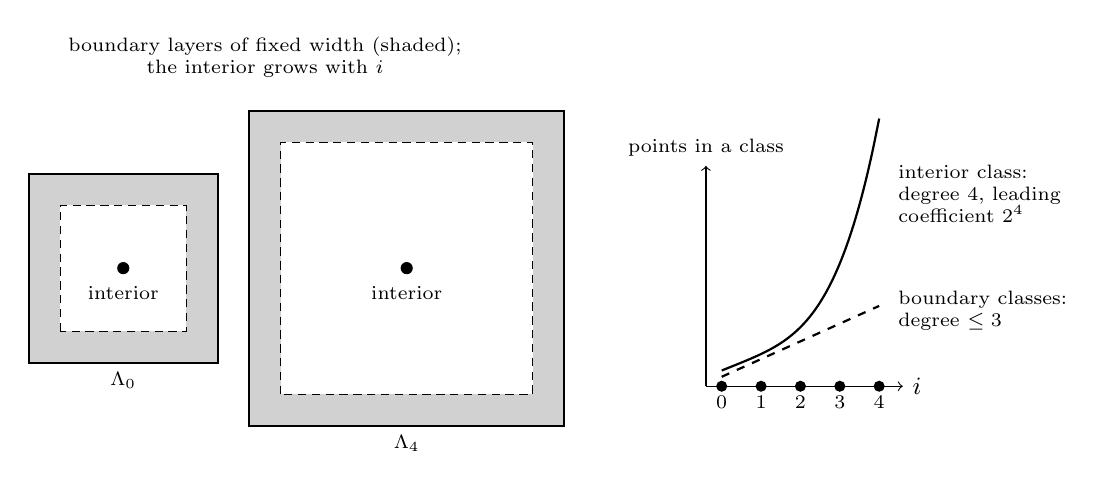
\begin{tikzpicture}[x=0.2cm,y=0.2cm,font=\small]
\foreach \h/\xs/\lab in {6/0/{$\Lambda_0$},10/18/{$\Lambda_4$}}{
  \begin{scope}[xshift=\xs*0.2cm]
  \fill[black!18] (-\h,-\h) rectangle (\h,\h);
  \fill[white] (-\h+2,-\h+2) rectangle (\h-2,\h-2);
  \draw[thick] (-\h,-\h) rectangle (\h,\h);
  \draw[densely dashed] (-\h+2,-\h+2) rectangle (\h-2,\h-2);
  \fill (0,0) circle (2.2pt);
  \node[font=\scriptsize] at (0,-1.6) {interior};
  \node[font=\scriptsize,below] at (0,-\h) {\lab};
  \end{scope}
}
\node[font=\scriptsize,align=center] at (9,13.4) {boundary layers of fixed width (shaded);\\ the interior grows with $i$};
\begin{scope}[xshift=7.4cm,yshift=-0.3cm]
\draw[->] (0,-6) -- (0,8) node[above,font=\scriptsize]{points in a class};
\draw[->] (0,-6) -- (12.5,-6) node[right]{$i$};
\foreach \i in {0,...,4} \fill (2.5*\i+1,-6) circle (2pt) node[below]{\scriptsize$\i$};
\draw[thick,domain=0:10,smooth,variable=\u] plot ({\u+1},{-5+12*(\u/10)^4+0.4*\u});
\draw[thick,dashed,domain=0:10,smooth,variable=\u] plot ({\u+1},{-5.4+0.45*\u});
\node[align=left,font=\scriptsize,anchor=west] at (11.6,6.2) {interior class:\\ degree $4$, leading\\ coefficient $2^4$};
\node[align=left,font=\scriptsize,anchor=west] at (11.6,-1.2) {boundary classes:\\ degree $\le3$};
\end{scope}
\end{tikzpicture}
\caption{The five reflected tori $\Lambda_i$ of Lemma~\ref{lem:D-localization}, of sides $2(w+i)$, drawn for $i=0$ and $i=4$. A point $y$ is classified by its local fold slopes and distances, through the read radius $R$, from reflection faces; on healthy $N_{2\bar w}(x)$, the shifted configurations $V_{i,x-\phi_i(y)}$ give the same local formula within each class. Boundary classes have multiplicity of degree at most three in $i$; the combined interior multiplicity has degree four and leading coefficient $2^4$. The fourth difference cancels the boundary classes and retains the interior contribution. The tori are auxiliary domains, and the cancellation takes place in the sum, not term by term.}
\label{fig:D-five-tori}
\end{figure}

Write $f_a^0$ for a regular summand of the negative logarithm in~\eqref{eq:D-cluster}, including its coefficient. Keep the inherited terms of Lemma~\ref{lem:D-inherited} separately. Call a remaining term \emph{low-order} if it is a connected term with at most two polymers of at most two elementary factors each, every path atom having length at most $B$, with no incoming activity factor or large-field component, or a path term of length at most $B$. Low-order terms read only the prescribed path, the coupling and the addresses, not the values of the incoming activities. Fix an exhaustion of the low-order addresses by finite sets invariant under translations and signed permutations, and select the low-order terms in one of these sets. Its index and the truncation error $\varepsilon_{\rm tr}$ are fixed in the proof of Lemma~\ref{lem:D-preliminary}. Give an ordinary term the shares $p_{xa}=\mathbf1_{X_a}(x)/|X_a|$, and a path term the share $\mathbf1_{\{o_a\}}(x)$; these shares sum to one. Put $F_x=\sum_{a\ {\rm selected}}p_{xa}f_a^0$, the selected low-order sum. The remaining terms form $f^{\rm tail}$. Let $R\ge1$ contain every complete read support of this finite sum relative to a site receiving a nonzero share, including all links read by its flag tests. The period argument below requires $R$ to be bounded by a fixed stage multiple of $1+B$ for the actual selected panel. The low-order factor count alone does not establish this for inverse or determinant defect chains; their read widths remain part of the verification in Lemma~\ref{lem:D-cutoff-continuity}. Set $w=4R+100(1+B)$, $\bar w=w+5$, and let $\Lambda_i$ have side $2(w+i)$, $0\le i\le4$. Use the fold $\phi_i$ and reflected configuration $V_{i,x}$ defined above. Put
\begin{equation}\label{eq:D-five-weights}
\lambda_i=\frac{(-1)^i\binom4i}{2^4\,4!},\qquad
G_x(V)=\sum_{i=0}^4\lambda_i\sum_{y\in\Lambda_i}F^{(i)}_y(V_{i,x})\,.
\end{equation}
Here $F^{(i)}$ is the same finite local formula on the auxiliary torus, with its value at $1$ subtracted at each site. The mask discrepancy and the constant of the redistribution are
\begin{equation}\label{eq:D-mask-localization}
L_x=\sum_{a\ \text{selected}}p_{xa}h_{X_a}f_a^0-F_x(1)
-\sum_{i=0}^4\lambda_i\sum_{y\in\Lambda_i}
 h_{N_{\bar w}(x-\phi_i(y))}F^{(i)}_y(V_{i,x-\phi_i(y)}),
\qquad c=F_0(1)\,,
\end{equation}
The shift is the folded position $\phi_i(y)$, not a torus representative.

For the estimates below put $\mathfrak b=\refbeta_{m+1}$; $P_j$ has subpower growth.
\begin{lemma}[Finite-period localization]\label{lem:D-localization}
The function $G_x$ is local on $N_{\bar w}(x)$, and
\begin{equation*}
\sum_a h_{X_a}f_a^0
=c|\Lambda|+\sum_a h_{X_a}f_a^{\rm tail}
+\sum_xh_{N_{\bar w}(x)}G_x+\sum_xL_x\,.
\end{equation*}
Each $L_x$ reads only links and flags in $N_{2\bar w}(x)$ and vanishes when that set is healthy, and
\begin{equation*}
\|G_x\|_{m,N_{\bar w}(x)}\le P_j(\mathfrak b)(\mathfrak b^{-23/20}+\varepsilon_{\rm tr}),
\qquad \sup|L_x|\le P_j(\mathfrak b)\mathfrak b^{-7/16}.
\end{equation*}
\end{lemma}
\begin{proof}
The identity is a rearrangement; the vanishing of $L_x$ is the fourth-difference cancellation; the bound on $G_x$ comes from the auxiliary logarithm, estimated with the classical and one-loop subtractions of Section~\ref{sec:partII-C}. For each $i,y$, translation by $\phi_i(y)$ is a bijection of the physical torus. Summing~\eqref{eq:D-mask-localization} over $x$ and changing $x$ to $x-\phi_i(y)$ gives exactly the asserted identity, including its masks. Translation symmetry makes $F_x(1)$ independent of $x$.

Use the polynomial period requirement in item~7 of Table~\ref{tab:constant-choices}, in addition to $100(B+1)\le L_pD_m$. Write $n=L_pD_m$. Subject to the stated stage-dependent bound on the actual read radius, $\bar w=4R+100(1+B)+5$ is bounded by a stage multiple $\bar a B/2$. The chosen stage has integers $v_j^{\rm per},h_j^{\rm per}$ with $v_j^{\rm per}\ge\bar a$, $h_j^{\rm per}\ge1$ and
\begin{equation*}
n\ge v_j^{\rm per}(1+B_m+B_{m+1})^{h_j^{\rm per}}.
\end{equation*}
These are the minimum-period choices made after the ratios. Since $B\ge1$,
\begin{equation*}
2\bar w\le\bar aB<\bar a(1+B_m+B_{m+1})^{h_j^{\rm per}}\le n,
\qquad 4R+16<n.
\end{equation*}
The reflection cubes, whose side is at most $2(w+4)<2\bar w$, therefore embed, as does every radius-$R$ read set. The larger health set $N_{2\bar w}(x)$ is a set on the original torus and need not embed; the argument uses only its containment of the queried links and flags.

For the local comparison, suppose that the field is healthy on the radius-$R$ neighbourhood. Translate its cube to $[0,2R]^4$. On integer representatives $0\le k<n$, fold each coordinate by $q(k)=k$ for $k\le2R$, $q(k)=4R-k$ for $2R<k\le4R$, and $q(k)=0$ thereafter. Pull back links along this map, reversing them on decreasing edges and setting them to the identity on collapsed edges. A plaquette becomes a plaquette of the original cube, with possible reversal and conjugation, or has identity holonomy. The field is therefore globally healthy and agrees with the original field on the cube. The bound $4R<n$ permits the construction without a divisibility assumption on $n$. Locality then permits this replacement when comparing the common local formulas on different periods.

We verify the vanishing of $L_x$ on a healthy $N_{2\bar w}(x)$. The complete read supports then lie in that set and every mask in~\eqref{eq:D-mask-localization} is one. At a site $y+u$ in the complete read, $\|u\|_\infty\le R$, the shifted reflected field reads the offset $\phi_i(y+u)-\phi_i(y)$ from~$x$, with inverse links on decreasing segments. This local profile depends only on the slope and on distances from the turning faces, including wrapped neighbours. Assign points at distance strictly less than $R$ from a face to boundary classes; each fixed boundary profile has a count independent of $i$. For each interior slope in one coordinate there are $h_i-2R+1$ sites with $R\le\phi_i(y)_a\le h_i-R$; there are two slopes. Multiplying the coordinate counts, every class meeting a boundary has multiplicity of degree at most three, while the combined interior multiplicity has leading coefficient $2^4$. Signed-permutation invariance identifies the values of the $2^4$ interior slope classes with $F_x(V)-F_x(1)$. The fourth difference therefore cancels all boundary classes and retains this value with coefficient one, proving $L_x=0$. Each shifted mask reads within $N_{2\bar w}(x)$ because $\|\phi_i(y)\|_\infty\le w+4<\bar w$.

\emph{Classification of the terms.} Here are the quantitative estimates on the sum before this localization. Put $\mathfrak b=\refbeta_{m+1}$ and $\mathfrak h=\mathfrak b^{3/8}$. In the convergent connected sums multiply the majorant of each ordinary elementary factor by $\mathfrak h$. The rooted attachment parameter still tends to zero, since $\mathfrak h \mathfrak b^{-7/16}=\mathfrak b^{-1/16}$. A term with at least three such factors across its polymers gains $\mathfrak h^{-3}$ upon restoring its original weights. A term with a retained large-field overlap has the same gain because its suppression is at least $\mathfrak h^{-3}$. The sum after multiplication has size at most a subpower factor times $\mathfrak h \mathfrak b^{-7/16}$. Thus the terms in these two classes have bound
\begin{equation}\label{eq:D-height-gain}
P_j(\mathfrak b)\mathfrak h^{-3}(\mathfrak h \mathfrak b^{-7/16})=P_j(\mathfrak b)\mathfrak b^{-19/16}
\le \mathfrak b^{-23/20}
\end{equation}
after the coupling threshold is raised. The reserve is $19/16-23/20=3/80$. This estimate also bounds fixed ordered derivatives: their placement polynomial was included before the rooted sum.

The connected sum separates into three parts. First retain the inherited terms using Lemma~\ref{lem:D-inherited}; their principal sum is made smaller than a prescribed multiple of $\epsilon^{\rm pre}_m$ by choosing the ratio, and their comparison remainder by raising the threshold. Among all other connected terms retain also those whose total support size exceeds the low-order radius: their support decay is at most $\mathfrak h^{-3}$ after the threshold is raised, so the estimate in~\eqref{eq:D-height-gain} applies to them. A term with an incoming regular factor and at least one further factor is not low-order. The rooted clause of Lemma~\ref{lem:D-connected}, with $W_\star$ that factor and at least one attached factor, bounds these terms by $P_j(\mathfrak b)\epsilon_{m+1}^{\rm reg}\mathfrak b^{-1/2}\le\mathfrak b^{-23/20}$. The remaining terms are low-order: the selected connected contributions and path terms of length at most $B$, to which the reflected-period construction is applied, and the low-order tail, of weighted norm at most $\varepsilon_{\rm tr}$. Long paths have an additional factor $e^{-w^{\rm path}_{J_m}B/4}$ by Lemma~\ref{lem:C1}; it converts their $\mathfrak b^{-7/16}$ bound to $\mathfrak b^{-23/20}$. Low-order connected terms with three or four elementary factors already obey~\eqref{eq:D-height-gain}; the remaining connected terms have at most two.

\emph{The auxiliary logarithm.} For the finite sum use the stationary integral on each $\Lambda_i$. Their sides $2(w+i)$ satisfy $2(w+i)\ge100(B+1)$. The entry choice $B\ge j+4$ also gives $\ell_m\,2(w+i)\ge100((j+3)\ell_m+1)$ for their fine periods. Thus the coarse-period form of Lemmas~\ref{lem:B-D1}--\ref{lem:B-D2} applies, without requiring these auxiliary periods to belong to the chosen physical-volume sequence. Subtract its flat value and the classical cubic, quartic and quadratic one-loop terms of Lemmas~\ref{lem:C4}--\ref{lem:C7}. Differentiation of its logarithm gives connected expectations under the common Gaussian law. For the terms not involving incoming errors, write the normalized local integral as $\mathbb E\exp(V_3+V_4+V_{\ge5})$, after the stationary action and its Gaussian determinant have been extracted. The subscripts refer to the Taylor degree in the link chart. Gaussian parity removes a lone odd cubic term. The fourth-order stationary terms are already in the classical path action, and the field-dependent quadratic part of the determinant is already in $\alpha\mathcal Q_m$ and the quadratic loop atoms. Subtracting the value at $1$ removes the remaining vacuum terms. Expanding $\log\mathbb E e^V$ through two factors gives $\mathbb EV+\frac12(\mathbb EV^2-(\mathbb EV)^2)$; its remaining terms have at least three factors. In normalized fluctuation coordinates each nonquadratic factor starts at order $\mathfrak b^{-1/2}$. The common Gaussian majorant bounds the last terms by $P_j(\mathfrak b)\mathfrak b^{-3/2}$. In the one- and two-factor terms that remain after the stated cancellations, Taylor's integral remainder and the healthy field bound give
\begin{equation*}
P_j(\mathfrak b)\{\mathfrak b^{-3/2}+\mathfrak b\,t_m^5+\mathfrak b^{-1}t_m+t_m^3+e^{-c_jB}\}
\le \mathfrak b^{-23/20}\,.
\end{equation*}
Every radius and chart loss is included in the subpower factor. Each of the four power terms has exponent at most $-3/2$ before that factor; the path exponential decreases faster than any fixed power. The quadratic subtraction uses the infinite-volume path coefficients, whereas the auxiliary logarithm uses the actual finite stationary branch. \hyperref[par:C-finite-period]{The finite-period recording paragraph} compares precisely these finite and periodized inputs. For $n_i=2(w+i)$ write its ordered-derivative error as
\begin{equation*}
\mathfrak e_i=C_{j,\ell_m}(1+\Lambda_{m+1}^{\rm loop})n_i^4P_{j,\ell_m}(n_i,B)e^{-c_{j,\ell_m}n_i}.
\end{equation*}
For the chart on the reflected configurations, choose paths from the origin in increasing coordinate order and gauge each bond by the paths to its endpoints. Commute a bond past the higher-coordinate path segments using at most $3(n_i-1)$ plaquette interchanges. A nonwrapping bond then cancels; for a wrapping bond the remaining coordinate cycle is the identity because the reflected extension traverses its links and then their reverses. Thus the gauge-fixed link chord is $O(n_it_m)$. Reflected perturbations retain the retracing property. Evaluate the exact gauge-invariant auxiliary functional and path subtraction in this smoothly chosen gauge before taking their flat Taylor expansions; the isolated quadratic expression in logarithms need not itself be invariant under a finite gauge change. Products of $O(n_i)$ links and the logarithm on a fixed ball around the identity have fixed-order derivatives bounded by a polynomial in $n_i$ and $B$. This construction concerns the auxiliary reflected configurations, not arbitrary healthy fields on a torus.

Here $P_{j,\ell_m}$ is a fixed polynomial for the ordered link derivatives and logarithmic-coordinate chain rules through the norm's prescribed order. The $n_i^4$ already bounds the whole torus quadratic form; no further site-count factor is applied to this error. Its flat value is zero, so centering leaves the quadratic difference unchanged. Differences between the nonlinear path representatives and their quadratic Taylor terms belong instead to the higher Taylor remainder displayed above. The comparison depends on the common analytic strip and its integrable bounds in \hyperref[par:C-finite-period]{the finite-period recording paragraph}; it also requires the reflected healthy torus to admit the coordinate charts and derivative bounds used for those chain rules. Both points remain under verification. At the fixed ratio, the stated bound on $n_i$ makes $\mathfrak e_i$ smaller than any prescribed inverse power of $\mathfrak b$. Terms involving incoming activities are not low-order; apart from the inherited terms they obey~\eqref{eq:D-height-gain} or the bound $P_j(\mathfrak b)\epsilon_{m+1}^{\rm reg}\mathfrak b^{-1/2}$ above. Subject to that finite-period comparison, Lemma~\ref{lem:B-D2} bounds these terms simultaneously, so the derivative bound for the centered total auxiliary sum is
\begin{equation}\label{eq:D-aux-bound}
C_j \mathfrak b^{-23/20}+\mathfrak e_i+2|\Lambda_i|\{C_j \mathfrak b^{-23/20}+\varepsilon_{\rm tr}\}\,.
\end{equation}
Here $\varepsilon_{\rm tr}>0$ is the chosen truncation error. The first term is the centered local integral, $\mathfrak e_i$ is the finite-period quadratic mismatch, and the two volume terms bound the omitted regular sum at the field and at $1$. Approaching a boundary point of the healthy domain by radial contraction preserves these estimates, so they hold on the closed domain used in Definition~\ref{def:D05a}.

A direction of that definition, restricted to $N_{\bar w}(x)$ and reflected, is bounded by $2t(1+\bar w)^{\varpi_{J_m}}$. Rescaling each of at most $\mathfrak q_{J_m}$ directions in~\eqref{eq:D-aux-bound} therefore gives
\begin{equation*}
\|G_x\|_{m,N_{\bar w}(x)}\le
2^{\mathfrak q_{J_m}}(1+\bar w)^{\varpi_{J_m}\mathfrak q_{J_m}}
\sum_{i=0}^4|\lambda_i|
 [C_j \mathfrak b^{-23/20}+\mathfrak e_i+2|\Lambda_i|(C_j \mathfrak b^{-23/20}+\varepsilon_{\rm tr})]\,.
\end{equation*}
All the factors outside the negative powers are fixed powers of $1+B$. Also $\cover_B(N_{\bar w}(x))$ is bounded by a stage constant. The regular bound divided by $\epsilon_m^{\rm reg}$ tends to zero, since $23/20>11/10$. Finally,~\eqref{eq:D-mask-localization} and the uncentered $\mathfrak b^{-7/16}$ bound give $\sup|L_x|\le P_j(\mathfrak b)\mathfrak b^{-7/16}$, with the same polynomial read radius. These logarithmic corrections tend to zero in the site norm at exponent $\sigma+2$ and vanish on healthy supports. Subject to the stated finite-period and sector inputs, these estimates give the bounds claimed for the localization.
\end{proof}

To specify the small coefficient, let $C_j^{\rm sub}$, $C_j^{\rm low}$ and $C_j^{\rm high}$ be the operator bounds for local subtraction, low path replacement and the part of high path replacement proportional to $\epsilon^{\rm pre}_m$. These are the three linear operations in the following subsections; they are fixed from the output derivative norm and path bounds. Put $C_j^0=C_j^{\rm sub}+C_j^{\rm low}+C_j^{\rm high}$. These constants use only derivative orders, direction powers, support exponents, and the output path bounds. For a prescribed $0<\theta\le1$, choose before the ratios
\begin{equation*}
c_j=\frac1{64(1+C_j^0)},\qquad \epsilon^{\rm pre}_m=\theta c_j\epsilon_m^{\rm reg}\,.
\end{equation*}
The quantity $\epsilon^{\rm pre}_m$ depends on $m$ through $\epsilon_m^{\rm reg}$. The next assertion concerns the very same block integral and the masks of~\eqref{eq:D-low-sums}. Its forced sum $\mathcal F_u^0$ is the disjoint-support exact-cover sum of Definition~\ref{def:D06} formed from the $k_{i,u}$, and $\mathfrak e_{i,u}\ge\|f_{i,u}\|_{m,X_i}$, $\mathfrak k_{i,u}\ge\sup_U|k_{i,u}(U)|$ are majorants.
\begin{lemma}[Preparatory activities]\label{lem:D-preliminary}
For every input curve above there are a continuous scalar $\tau_u$, local regular functions $f_{i,u}$, with the regularity of Definition~\ref{def:D24} before flat-value and Hessian subtraction, and forced activities $k_{i,u}$ (Definition~\ref{def:D25}), all with fixed addresses, equivariant and continuous in the weighted norms with exponents $\sigma+3$ and $\sigma+1$, such that
\begin{align}\label{eq:D-early}
\mathcal H_u(U)&=e^{\tau_u|\Lambda|-\beta'_u\mathsf K_m^{\rm kin}(U)-\mathcal L_m(U)
-\alpha_{N,m}\mathcal Q_m(U)-\sum_i h_{X_i}(U)f_{i,u}(U)}\mathcal F_u^0(U),\\
\sup_x\sum_{o_i=x}e^{(\sigma+3)\cover_B(X_i)}\mathfrak e_{i,u}&\le\epsilon^{\rm pre}_m,\label{eq:D-early-bound}\\
\sup_x\sum_{i:x\in Y_i}e^{(\sigma+1)\cover_B(Y_i)}\mathfrak k_{i,u}&\le e^{-\kappa_j^{\rm pre}(\cutoffsize_{m+1})^2},
\label{eq:D-preliminary-forced}
\end{align}
with $\kappa_j^{\rm pre}>0$ fixed after the ratio. Restricting the interval preserves all this.
\end{lemma}
\begin{proof}
The connected expansion of Lemma~\ref{lem:D-connected} supplies the terms, Lemma~\ref{lem:D-inherited} and the classification in the proof of Lemma~\ref{lem:D-localization} bound all but the low-order ones, and Lemma~\ref{lem:D-localization} localizes the latter; the choices below split $\epsilon^{\rm pre}_m$ among them. First choose the ratio so that the inherited principal terms of Lemma~\ref{lem:D-inherited} use at most $\epsilon^{\rm pre}_m/32$, and then raise the threshold so that their comparison remainders use at most $\epsilon^{\rm pre}_m/32$. Bound the terms retained in~\eqref{eq:D-height-gain} and the long paths together by $\epsilon^{\rm pre}_m/16$. The localization bound is $o(\epsilon^{\rm pre}_m)$ with the stronger support exponent. This fixes a coupling threshold independent of the period.

Next fix the truncation index. The low-order tail reads only the prescribed path, the coupling and the incoming addresses. For each coupling in $\mathfrak B_{m+1}$ summability gives a tail smaller than $\varepsilon_{\rm tr}/2$; weighted continuity in the coupling gives a neighbourhood on which the same tail is smaller than $\varepsilon_{\rm tr}$. Finitely many neighbourhoods cover the compact $\mathfrak B_{m+1}$; take the largest index. This argument gives an index for a fixed prescribed path and address lists. The cutoff comparison requires additional uniform control of the actual selections, including defect-chain tails, as specified in Lemma~\ref{lem:D-cutoff-continuity}. Increasing a valid index preserves its tail bound. Choose the tail bound to be at most $\epsilon^{\rm pre}_m/16$. The regular terms outside the finite sum then have total at most $(1/16+2/16)\epsilon^{\rm pre}_m$. Choose $\varepsilon_{\rm tr}$ so that the two localization errors in~\eqref{eq:D-aux-bound}, including the direction and support losses, have total at most $12\epsilon^{\rm pre}_m/16$. The resulting bound is $15\epsilon^{\rm pre}_m/16<\epsilon^{\rm pre}_m$.

The change in the scalar is $\tau_u^{\rm old}-F_0(1)$, with the sign fixed by~\eqref{eq:D-mask-localization}. Multiply the preliminary forced sum by $\exp(-\sum_xL_x)$. Expand each $e^{-L_x}$ about one and collect intersecting supports, as in the proof of Lemma~\ref{lem:D-fusion}. The logarithmic factors vanish unless their supports contain flags, so each resulting connected component still contains a forced term. Their site bound at exponent $\sigma+2$ is a subpower factor times $\mathfrak b^{-7/16}$, whereas each forced component retains $C_j e^{-r_j\beta'_u t_{m+1}^2}$. Choose a smaller positive $r'_j<r_j$. The site attachment parameter tends to zero and the remaining exponential gives
\begin{equation*}
C'_j e^{-r'_j\beta'_u t_{m+1}^2}
\le e^{-\kappa_j^{\rm pre}(\cutoffsize_{m+1})^2}
\end{equation*}
for some $\kappa_j^{\rm pre}>0$, since $\beta'_u\ge\refbeta_{m+1}/2$. One extra support power is used in this collection, leaving $\sigma+1$. Lemma~\ref{lem:D-rooted} proves the asserted site bound and absolute convergence. No scalar depends on the output configuration, and all identities hold also when a chord is exactly at a threshold.

For continuity, the truncation and all reflected tori are now fixed. Finite linear combinations preserve the weighted comparison from Lemma~\ref{lem:D-connected}. A difference of forced products has one marked difference factor; the rooted sum has the same strict attachment margin. Dominated convergence proves the weighted comparison after the collection. Flat evaluation gives continuity of the scalar. The support enlargement, inventories and conjunctions of tests are fixed. The same constructions commute with translations and signed permutations by reindexing. Every assertion is pointwise in the interval parameter or a convergence assertion within the interval, so restriction to a closed subinterval preserves it.
\end{proof}


The preparatory regular sum is $E_u^{\rm pre}=\sum_i f_{i,u}$ on the healthy domain. Its weighted bound is the anchored sum of Definition~\ref{def:D05b}, before flat-value and Hessian subtraction. The next identity supplies the scalar reset.

\begin{lemma}[Pre-reset expansion]\label{lem:D4}
For every input curve above and every $u$, there is a preparatory regular family with sum $E_u^{\rm pre}$ and weighted bound $\epsilon_m^{\rm reg}$ such that, when $\flags_m(U)=\varnothing$,
\begin{equation*}
\mathcal H_u(U)=\exp\{\tau_u|\Lambda|-\beta'_u\mathsf K_m^{\rm kin}(U)
-\alpha_{N,m}\mathsf K_{2,m}^{\rm kin}(U)-\mathcal L_m(U)-E_u^{\rm pre}(U)\}\,.
\end{equation*}
In particular $\mathcal H_u(1),\mathcal H_u(U)>0$ on this set.
\end{lemma}

\begin{proof}
Restrict the identity~\eqref{eq:D-early} to configurations without flags. Set $E_u^{\rm pre}=\sum_i f_{i,u}$ on configurations without flags. Every health mask is one, and nonempty forced inventories give $\mathcal F_u^0=1$. Equation~\eqref{eq:D-low-sums} gives $\mathcal Q_m=\mathsf K_{2,m}^{\rm kin}$. Dropping the extra three support powers gives the stated bound, since $\theta c_j\le1/64$. Absolute convergence makes the exponent finite and real, proving positivity, including at $1$. 
\end{proof}

\subsection{Local quadratic subtraction}\label{subsec:D-subtraction}

The subtraction is local and uses no bound on the eventual coupling correction. It extracts from each preliminary regular function its response to constant curls, written with the clover curvature of~\eqref{eq:D-clover-linear}.

For a preliminary $f$ on $X$ anchored at $o$, put $Z=X\cup N_2(o)$. For $q=(a,b)$ and $T\in\g$, set $A^{q,T}_{(y,c)}=\mathbf1_{c=b}\xi_o(y)^aT$, and fix a unit vector $T_*\in\g$. Define
\begin{align*}
q_f(q,r)&=D^2[f(\exp\cdot)](0)[A^{q,T_*},A^{r,T_*}],\\
Q_f(U)&=\frac12\sum_{q,r}q_f(q,r)\langle F^{\rm cl}_q(U,o),F^{\rm cl}_r(U,o)\rangle_{\g}\,.
\end{align*}
Set $q_f=0$ when $Z$ wraps. The matrix extracts the response to constant curls; its color independence is proved below. Define the regular remainder and the discrepancy of masks by
\begin{align}\label{eq:D-local-split}
R_f&=f-f(1)-Q_f,\notag\\
\zeta_f&=\mathbf1_{Z\,\mathrm{unhealthy}}\{f(1)+h_{\{o\}}Q_f-h_Xf\}\,.
\end{align}
The following identity is checked before any activities are summed.

\begin{lemma}[Local subtraction]\label{lem:D-local-subtraction}
For every preliminary regular $f$,
\begin{equation*}
h_Xf=f(1)+h_{\{o\}}Q_f-\zeta_f+h_ZR_f\,.
\end{equation*}
The function $R_f$ is regular on $Z$, vanishes at $1$, and has zero affine Hessian when $Z$ is nonwrapping. The Borel gauge-invariant function $\zeta_f$ depends only on internal links and flags in $Z$ and vanishes when $Z$ is healthy.
\end{lemma}

\begin{proof}
Gauge invariance reduces the affine Hessian to its response to constant curls, Schur's lemma makes that response colour-independent, and the clover formula~\eqref{eq:D-clover-linear} reproduces it. The first derivative of $f$ at the flat field vanishes: constant gauge transformations make its coefficient on each internal link an adjoint-invariant vector of $\g$, hence a central vector, which is zero. Differentiating local gauge invariance again makes its Hessian annihilate an infinitesimal gradient in either argument. On a nonwrapping support an affine field with zero curl is a local gradient. Its constant and symmetric linear parts are differences of a quadratic site field, with a constant adjustment for the discrete difference. Multiply this site field by a periodic cutoff equal to one on $Z$. The internal links read by $f$ are unchanged. The second differentiation of gauge invariance uses $Df(1)=0$, as proved above, so no second derivative of the gauge orbit remains. Hence the affine Hessian depends only on the constant curls.

For each pair of orientations the colour form $(S,T)\mapsto D^2[f(\exp\cdot)](0)[A^{q,S},A^{r,T}]$ is $\operatorname{Ad}(G)$-invariant. The complexified adjoint representation of the compact simple Lie algebra $\g$ is irreducible, so every invariant bilinear form on $\g$ is a multiple of the trace form (Schur's lemma); testing on $T_*$ identifies the multiple.

The side satisfies $L_pD_m\ge100(B_m+1)>20$, which permits the clover loops and affine tests without degeneracies. Equation~\eqref{eq:D-clover-linear} identifies the affine Hessian of $Q_f$ with that of $f$. Subtracting gives zero diagonal affine Hessian for $R_f$; polarization gives zero on pairs. The value and first derivative of $R_f$ vanish at $1$. If $Z$ wraps, no Hessian cancellation is required. The clover polynomial is smooth, Borel, gauge invariant and local on $N_2(o)$, which gives the other regularity assertions on $Z$.

All indicators in $\zeta_f$ read flags in $Z$. If $Z$ is healthy, every mask in the identity is one and $\zeta_f=0$; the identity reduces to the definition of $R_f$. If $Z$ is unhealthy, $h_ZR_f=0$ and the definition of $\zeta_f$ gives the identity directly. This proves the equality on every configuration and the stated locality and cancellations.
\end{proof}

The same subtraction has a quantitative bound. If $a_f$ majorizes $f$, the diagonal tests $tA^{q,T_*}$ and their half-sum are permitted directions in Definition~\ref{def:D05a}. They give
\begin{equation}\label{eq:D-projection-bound}
t^2|q_f(q,q)|\le a_f,\qquad t^2|q_f(q,r)|\le3a_f\,.
\end{equation}
Indeed four times the half-sum's diagonal Hessian is $t^2(q_f(q,q)+q_f(r,r)+2q_f(q,r))$. Its absolute value and the two diagonal bounds give the second estimate. Product differentiation of the four-link formula bounds every permitted derivative of $F^{\rm cl}_q$ by $C_jt$ at a healthy anchor. For order zero this follows from the plaquette chord bound; at positive order the direction factors supply $t$, and all undifferentiated group matrices are bounded. Hence
\begin{equation}\label{eq:D-remainder-bound}
\|R_f\|_{m,Z}+\sup_U|\zeta_f(U)|\le C_j a_f\,.
\end{equation}
For $\zeta_f$, the terms $Q_f$ and $f$ occur only under their own relaxed threshold tests, so the estimates still apply when $Z$ is unhealthy.

Enlargement satisfies $\cover_B(Z)\le\cover_B(X)+1$: one radius-$B$ ball centered at $o\in X$ contains $N_2(o)$ and meets the original connected cover. Also $\operatorname{dist}(x,o)\le C B\cover_B(Z)$ for $x\in Z$, by following the connected cover. For a support of covering number $n$ through $x$, its anchor lies within distance $C Bn$ of $x$, giving at most $C(1+B)^4(1+n)^4$ possible anchors. The inequality $(1+n)^4\le C e^n$ converts exponent $\sigma+3$ at the anchor to exponent $\sigma+1$ at a site: one support power bounds this polynomial and one remains unused. At exponent $\sigma$ the enlargement itself contributes only a stage constant. Without these extra powers the conversion would leave a polynomial in $n$ at the original exponent.

Sum $q_{f_{i,u}}$ at each anchor. Translation covariance makes the result independent of the anchor. Reflection in an axis belonging to exactly one of two distinct orientations changes the sign of the off-diagonal entry, so that entry is zero. Permuting axes identifies the diagonal entries. Thus a single real $\Delta_u$ satisfies
\begin{align}\label{eq:D-isotropy}
\sum_{o_i=o}q_{f_{i,u}}(q,r)&=\Delta_u\delta_{qr},\notag\\
\sum_i h_{\{o_i\}}Q_{f_{i,u}}
&=\frac{\Delta_u}2\sum_o h_{\{o\}}\sum_q|F^{\rm cl}_q(U,o)|^2\,.
\end{align}
The coefficient sums converge absolutely by~\eqref{eq:D-projection-bound}, and $t^2|\Delta_u|\le\epsilon^{\rm pre}_m$. In particular $|\Delta_u|\le\epsilon^{\rm pre}_m/t_m^2=\theta c_j\refbeta_m^{-1/10}(\cutoffsize_m)^{-2}<1$, since $\theta c_j\le1/64$, $\refbeta_m>1$ and $\cutoffsize_m\ge1$. This is already the numerical reset bound, and with Lemma~\ref{lem:C7} it gives the drift bound of Lemma~\ref{lem:C8} directly; no further restriction enters. The probe argument in the proof of Lemma~\ref{lem:C8} is a second proof of $|\Delta_u|\le1$ with a separate role: it reads $\Delta_u$ off the two numbers $\mathcal H_u(1),\mathcal H_u(V)$ as the unique root of an affine equation, without the formula~\eqref{eq:D-isotropy}. Hence no other coupling correction fits the same activities, and $\Delta_u$ is continuous in~$u$ because the block integral and the activity sums are (Lemma~\ref{lem:D6}).

\subsection{Forced fusion, activity bounds and the reset}\label{subsec:D-fusion}

Put $\alpha=\alpha_{N,m}$. After Section~\ref{subsec:D-subtraction} the exponent contains $\alpha\mathcal Q_m+\frac{\Delta_u}2\sum_oh_{\{o\}}\sum_q|F^{\rm cl}_q(U,o)|^2$, whereas the output density must contain $(\alpha+\Delta_u)\mathsf K^{\rm kin}_m$. The difference consists of clover versus plaquette curvature, the missing cubic and quartic atoms, and the clips and health masks. The first two become regular activities, $e_{\lambda,u}$ below and $-(\alpha+\Delta_u)\mathfrak a^{(k)}_i$; the third, $\ell_{\lambda,u}$, vanishes on healthy supports and, with the mask discrepancies $\zeta_f$ of Lemma~\ref{lem:D-local-subtraction}, is absorbed into the forced activities by Lemma~\ref{lem:D-fusion}. Define
\begin{align}\label{eq:D-kinetic-split}
e_{\lambda,u}&=\Delta_u(L^{\rm cl}_\lambda-L^{\rm raw}_\lambda),\notag\\
\ell_{\lambda,u}&=(\alpha+\Delta_u)(L_\lambda-h_{Z_\lambda}L^{\rm raw}_\lambda)
+\Delta_u(h_{Z_\lambda}-h_{\{o_\lambda\}})L^{\rm cl}_\lambda\,.
\end{align}
The regular function is used with mask $h_{Z_\lambda}$. Its affine Hessian vanishes because its two terms have the same constant-curl response. Add also the regular cubic and quartic functions $-(\alpha+\Delta_u)\mathfrak a_i^{(k)}$, with their prescribed masks; they have zero Hessian because $k\ge3$. Every $\ell_{\lambda,u}$ vanishes on healthy $Z_\lambda$.

Write the logarithmic corrections $\zeta_{f_{i,u}}$ and $\ell_{\lambda,u}$ as $\ell_a$ on nonempty supports $Z_a$. A connected selection $P$ consists of preliminary forced labels and logarithmic labels, contains at least one forced label, and has pairwise disjoint preliminary forced supports. Connected means connected in the graph joining intersecting supports. Its support $Y_P$ is the union of all supports, including logarithmic supports; its inventory $I_P$ is the union of the preliminary forced inventories. Define
\begin{equation}\label{eq:D-fused-term}
K_P(U)=\mathbf1_{\{Y_P\cap\flags_m(U)=I_P\}}
\prod_{i\in P_{\rm for}}k_{i,u}(U)
\prod_{a\in P_{\rm log}}(e^{\ell_a(U)}-1)\,.
\end{equation}
The extra test is the conjunction of the preliminary forced tests. Selections and tests are fixed as $u$ varies.

\begin{lemma}[Forced fusion]\label{lem:D-fusion}
Suppose $\sum_a\sup_U|\ell_a(U)|<\infty$. For $\kappa_{\rm fus},\gamma\ge0$ assume nonnegative $v_a$ for all forced and logarithmic labels with
\begin{equation*}
|k_i|\le e^{-\kappa_{\rm fus}}v_i,\quad |e^{\ell_a}-1|\le v_a,\quad
\sup_x\sum_{a:x\in Z_a}e^{(\sigma+1)\cover_B(Z_a)}v_a\le\gamma,
\quad(2B+1)^4\gamma\le1\,.
\end{equation*}
Then the exact-cover gas of~\eqref{eq:D-fused-term} equals $\mathcal F_u^0\exp(\sum_a\ell_a)$ and its forced norm of Definition~\ref{def:D05b} is at most $e^{-\kappa_{\rm fus}}(e^\gamma-1)$.
\end{lemma}

\begin{proof}
The identity is a regrouping of finite selections into overlap components; the bound is Lemma~\ref{lem:D-rooted}. Expand $\exp(\sum_a\ell_a)=\prod_a(1+(e^{\ell_a}-1))$. Decompose a finite selection, together with a selection from $\mathcal F_u^0$, into support-overlap components. A nonzero logarithmic factor meets a flag. Exact coverage assigns that flag to a preliminary forced label, whose support meets the logarithmic support. Every component therefore contains a forced label. Their union supports are disjoint; their union inventories cover all flags. Conversely the components recover the original selection uniquely. The eligibility indicator in~\eqref{eq:D-fused-term} equals one on any such nonzero product: another component cannot supply a flag in $Y_P$, since its support is disjoint. This proves the identity for finite expansions.

For the absolute bound retain $e^{-\kappa_{\rm fus}}$ from one forced label per connected selection. Apply Lemma~\ref{lem:D-rooted}, with $\eta=1$, to the weights $\mathfrak v_i=v_ie^{\sigma\cover_B(Z_i)}$; its hypothesis follows from $(2B+1)^4\gamma\le1$ and the extra exponent in the hypothesis here. It bounds the rooted tree sums by $\mathfrak v_ie^{\cover_B(Z_i)}$, and the sum of these bounds over roots whose supports contain a fixed site is at most $\gamma$. Every connected selection has a spanning tree rooted at a label whose support contains that site, so its sum is at most $\gamma\le e^\gamma-1$. The covering number is subadditive on intersecting unions, which retains $e^{\sigma\cover_B(Y_P)}$ in this comparison. Restoring $e^{-\kappa_{\rm fus}}$ gives the claimed bound. The resulting summable envelope justifies passage from finite expansions to the infinite identity.
\end{proof}

Let $E_u^{\rm sum}$ be the masked sum of the $R_{f_{i,u}}$, the $e_{\lambda,u}$, and the cubic and quartic corrections. Let $\mathcal F_u$ be the fused gas. Hold these functions fixed while a trial parameter $\vartheta$ varies, and put
\begin{equation*}
q_{u,\vartheta}=e^{-(\beta'_u+\alpha_{N,m}+\vartheta)\mathsf K_m^{\rm kin}-\mathcal L_m-E_u^{\rm sum}}\mathcal F_u\,.
\end{equation*}
The parameter $\vartheta$ is the free coupling correction of the scalar reset. Lemma~\ref{lem:D5} shows that $\vartheta=\Delta_u$ gives the density identity at every configuration; at one healthy test configuration $V$ with $\mathsf K^{\rm kin}_m(V)>0$, Lemma~\ref{lem:C8} uses the affine dependence on $\vartheta$ to read off $\Delta_u$, which gives its continuity in $u$ and, with Lemma~\ref{lem:C7}, the drift bound.
The output representation is the following single list: regular addresses $(Z_i,o_i)$ with functions $R_{f_{i,u}}$, addresses $(Z_\lambda,o_\lambda)$ with functions $e_{\lambda,u}$, the cubic and quartic addresses of Definition~\ref{def:D22} with functions $-(\alpha+\Delta_u)\mathfrak a_i^{(k)}$, and forced addresses $(Y_P,I_P,\mathcal E_P^{\rm extra})$ with functions $K_P$. Each regular function carries its own health mask. We prove the inequalities
\begin{equation}\label{eq:D-fusion-small}
e^{-\kappa_{\rm fus}}(e^\gamma-1)\le\epsilon_m^{\rm for},\qquad
\mathcal E_m\le\epsilon_m^{\rm reg}\,.
\end{equation}
in Lemma~\ref{lem:D1} before using them for the density identity. They impose no condition on the trial coupling.

\begin{lemma}[Activity bounds and covariance]\label{lem:D1}
For every coarse output constructed above, both activity families are countable and equivariant under translations and $\hypercubic$, including supports, anchors, inventories and tests. There exist nonnegative majorants as in Definitions~\ref{def:D05a}--\ref{def:D05b} whose weighted series converge and which satisfy
\begin{equation*}
\mathcal E_m\le\epsilon_m^{\rm reg},\qquad
\mathcal K_m\le\epsilon_m^{\rm for}\,.
\end{equation*}
\end{lemma}
Lemma~\ref{lem:D3} states the same bounds for the Wilson representation, and Lemma~\ref{lem:D2} extends them to all the chosen classes.


\begin{proof}[Proof for a coarse output]
The regular bound adds the contributions of the three linear operations to the preparatory bound of Lemma~\ref{lem:D-preliminary}; the forced bound applies Lemma~\ref{lem:D-fusion}. Equation~\eqref{eq:D-remainder-bound} controls each subtracted function. The low regular terms are bounded by $C_j\epsilon^{\rm pre}_m$, since $t^2|\Delta_u|\le \epsilon^{\rm pre}_m$. The high terms are bounded by $C_j(|\alpha|t^3+\epsilon^{\rm pre}_m)$: each has at least three curvature factors, and $|\Delta_u|t^3\le \epsilon^{\rm pre}_mt\le \epsilon^{\rm pre}_m$. A derivative of a word of length $l$ introduces a fixed power of $1+l$, by the product rule and the allowed spatial growth of the directions. The support obeys $\cover_B(Z_\lambda)\le C+l/B$. Raise the threshold until $\sigma/B\le w^{\rm path}_{J_m}/4$. A quarter of the path exponent then bounds the support weight, and another quarter bounds this polynomial, since $\sup_{l\ge0}(1+l)^ke^{-wl/2}<\infty$. Summing Lemma~\ref{lem:C1} gives the previously defined constant $C_j^0$ and a constant $C_j^1$ with
\begin{equation*}
\mathcal E_m\le C_j^0\epsilon^{\rm pre}_m+C_j^1|\alpha|t^3\,.
\end{equation*}
The constant $c_j=[64(1+C_j^0)]^{-1}$ was chosen before the ratios in Lemma~\ref{lem:D-preliminary}. After the ratio is fixed, Lemma~\ref{lem:C7} bounds $|\alpha|$; raise the entry threshold until $C_j^1|\alpha|t^3\le\epsilon_m^{\rm reg}/2048$. This is possible because $t^3/\epsilon_m^{\rm reg}=\refbeta_m^{-2/5}(\cutoffsize_m)^3\to0$. Take $\theta\le1/32$ before the ratio. Since $C_j^0c_j\le1/64$, the sum is at most $\epsilon_m^{\rm reg}/1024$. The same argument allows any prescribed smaller coefficient by choosing $\theta$ first and raising the threshold for the second term.

For the logarithmic corrections, conversion from anchored sums to site sums introduces at most $C_j(1+B)^4$, after the extra support powers absorb the powers of the covering number. The local subtraction is bounded by $C_j\epsilon^{\rm pre}_m$. The low terms in~\eqref{eq:D-kinetic-split} are bounded by
\begin{equation*}
C_j(1+B)^4\{(|\alpha|+\epsilon^{\rm pre}_m/t^2)t+\epsilon^{\rm pre}_m\}=:m_j\,.
\end{equation*}
The linear clipped tail is bounded by $2c_{\rm lin}t$ times its coefficient, since chords are at most two. For a failed relaxed threshold test, the remote threshold supplies $e^{l/R_{J_m}^{\rm rel}}$ in a path of length $l$. The path decay absorbs it because $R_{J_m}^{\rm rel}w_{J_m}^{\rm path}\ge12$. The common-anchor clover term is bounded by $|\Delta_u|t^2\le \epsilon^{\rm pre}_m$. These estimates give exactly the displayed bound, including unhealthy configurations. Since $\epsilon^{\rm pre}_m/t=O_j(\refbeta_m^{-3/5}/\cutoffsize_m)$ and $|\alpha|$ is fixed after the ratio, $(1+B)^4m_j\to0$.

Let $\kappa_{\rm fus}=\kappa_j^{\rm pre}(\cutoffsize_{m+1})^2/2$. The majorants in~\eqref{eq:D-preliminary-forced}, multiplied by $e^{\kappa_{\rm fus}}$, have rooted total at most $e^{-\kappa_{\rm fus}}$. For each logarithm use $|e^{\ell_a}-1|\le2|\ell_a|$ once its individual majorant is at most $\log2$; this follows by increasing the entry threshold until $m_j\le\log2$. Their rooted total is at most $2m_j$. Increase the entry threshold so that $(2B+1)^4\gamma\le1/2$ for $\gamma=e^{-\kappa_{\rm fus}}+2m_j$. Lemma~\ref{lem:D-fusion} applies. Increase the threshold further so that $\gamma\le1$ and $e^{-\kappa_{\rm fus}}(e^\gamma-1)\le\epsilon_m^{\rm for}/1024$. Indeed $e^\gamma-1\le2\gamma$ and $\kappa_{\rm fus}\gg(\cutoffsize_m)^{1/5}$. This proves the forced inequality and summability in~\eqref{eq:D-fusion-small}.

Every address is a finite combination of countable preliminary and path addresses, so the families are countable. Subtraction and path replacement transport the entire address under translations. Signed permutations transform the curvature orientations with their signs; the finite group average includes every transformed term. These permutations act on supports, anchors and functions. On a connected selection they also transform the union inventory and conjunction of tests. Equation~\eqref{eq:D-fused-term} therefore has the required covariance. For an inverse link, $(e^{zA}U)^{-1}=e^{-z\operatorname{Ad}_{U^{-1}}A}U^{-1}$. Differentiating this identity repeatedly gives only finitely many product-rule terms through order $\mathfrak q_{J_m}$; the adjoint-invariant norm bounds them by a constant depending on that order. This proves the complete address covariance and the convergent weighted bounds for a coarse output. The Wilson start is established below; induction in Lemma~\ref{lem:D2} then gives the class assertion.
\end{proof}

The identity below fixes the whole density before the scalar estimate of Lemma~\ref{lem:C8}. Its proof uses the bounds just established.
\begin{lemma}[Exact density representation]\label{lem:D5}
The final activities satisfy Lemma~\ref{lem:D1}, vanish at the flat field in their regular part, and are independent of $\vartheta$. For every $u$ there is $\Delta_u\in\R$ such that
\begin{equation*}
q_{u,\Delta_u}(U)=\frac{\mathcal H_u(U)}{\mathcal H_u(1)}
\qquad\text{for every }U\,.
\end{equation*}
Moreover $\mathcal F_u(U)=1$ when $\flags_m(U)=\varnothing$. 
\end{lemma}

\begin{proof}
Local subtraction rewrites the preliminary regular functions, path replacement turns the masked quadratic functional into the kinetic action, and fusion absorbs the logarithmic corrections; the bounds~\eqref{eq:D-fusion-small} make every sum converge. Choose $\Delta_u$ by~\eqref{eq:D-isotropy} and put $c_u=\sum_i f_{i,u}(1)$. Local subtraction gives
\begin{equation*}
\sum_i h_{X_i}f_{i,u}=c_u+\frac{\Delta_u}2\sum_o h_{\{o\}}\sum_q|F^{\rm cl}_q|^2
-\sum_i \zeta_{f_{i,u}}+\sum_i h_{Z_i}R_{f_{i,u}}\,.
\end{equation*}
All sums converge absolutely. For each low term~\eqref{eq:D-kinetic-split} gives
\begin{equation*}
\begin{aligned}
&(\alpha+\Delta_u)L_\lambda+\Delta_u h_{Z_\lambda}(L^{\rm cl}_\lambda-L^{\rm raw}_\lambda)-\ell_{\lambda,u}\\
&\qquad=\alpha h_{Z_\lambda}L^{\rm raw}_\lambda+\Delta_u h_{\{o_\lambda\}}L^{\rm cl}_\lambda\,.
\end{aligned}
\end{equation*}
Sum and apply~\eqref{eq:D-low-sums}. The high corrections cancel $(\alpha+\Delta_u)\mathcal A_m$. Thus the exponent in~\eqref{eq:D-early} becomes
\begin{equation*}
\begin{aligned}
&(\tau_u-c_u/|\Lambda|)|\Lambda|
-(\beta'_u+\alpha+\Delta_u)\mathsf K_m^{\rm kin}-\mathcal L_m-E_u^{\rm sum}\\
&\qquad+\sum_i \zeta_{f_{i,u}}+\sum_\lambda\ell_{\lambda,u}\,.
\end{aligned}
\end{equation*}
Lemma~\ref{lem:D-fusion} incorporates the last two sums into $\mathcal F_u$. Hence, on every configuration,
\begin{equation}\label{eq:D-unnormalized}
\mathcal H_u(U)=e^{(\tau_u-c_u/|\Lambda|)|\Lambda|}q_{u,\Delta_u}(U)\,.
\end{equation}
At $1$ all path and final regular terms vanish. The only exact-cover forced selection is empty, so $q_{u,\vartheta}(1)=1$ for every $\vartheta$. Equation~\eqref{eq:D-unnormalized} proves the quotient identity and positivity of its denominator. The same empty-selection argument gives $\mathcal F_u=1$ whenever there are no flags.

The regular cancellations were proved in Lemma~\ref{lem:D-local-subtraction} and after~\eqref{eq:D-kinetic-split}; the weighted bounds are those of Lemma~\ref{lem:D1}. The value $\Delta_u$ used in the activity construction is already fixed by the preliminary functions. The trial variable $\vartheta$ occurs only in the exponential defining $q_{u,\vartheta}$. This proves the exact identity without using Lemma~\ref{lem:C8} or its reset estimate.
\end{proof}

\paragraph{The scalar reset.}\label{subsec:C-reset}

The density identity of Lemma~\ref{lem:D5} holds with a value $\Delta_u$ that the construction fixes before the bound on it proved here is used. The proof order is
\begin{equation*}
\begin{tikzpicture}[baseline=(c.base),node distance=0.45cm,every node/.style={draw,rounded corners=2pt,align=center,font=\footnotesize,inner sep=3pt}]
\node (a) {fixed path\\arrays\\(Section~\ref{sec:partII-C})};
\node[right=of a] (b) {activities and exact\\trial identity\\(Lemma~\ref{lem:D5})};
\node[right=of b] (c) {probe contrast at $V$,\\no bound on $\Delta_u$\\assumed};
\node[right=of c] (d) {bounded reset\\and drift\\(Lemma~\ref{lem:C8})};
\node[right=of d] (e) {admissible\\recursion\\(Section~\ref{subsec:D-recursion})};
\foreach \x/\y in {a/b,b/c,c/d,d/e} \draw[->,thick] (\x) -- (\y);
\end{tikzpicture}
\end{equation*}
Before the estimate below the following are available: the path arrays and $\alpha_{N,m}$ (Section~\ref{sec:partII-C}), the activity families with their bounds (Lemma~\ref{lem:D1}), and the exact identity $q_{u,\Delta_u}=\mathcal H_u/\mathcal H_u(1)$ (Lemma~\ref{lem:D5}). Section~\ref{subsec:D-subtraction} already gives $t_m^2|\Delta_u|\le\epsilon^{\rm pre}_m$, which the activity bounds use and which alone implies $|\Delta_u|<1$ and the drift bound. The estimate below is an alternative proof of $|\Delta_u|\le1$ that uses the activity bounds but not the formula for~$\Delta_u$. The reset gives a second description of the same coefficient: evaluating the identity at one configuration with positive kinetic energy identifies $\Delta_u$ as the unique root of an affine scalar equation. This explicit formula, with the continuity of Lemma~\ref{lem:D6} in Section~\ref{subsec:D-continuity} (whose proof does not use Lemma~\ref{lem:C8}), gives the continuity of $\Delta_u$ in $u$; with Lemma~\ref{lem:C7} it gives the drift bound.

For an input curve $\rho'_u$ of Theorem~\ref{prop:RG}, recall $\mathcal H_u=\blockmap{m}_{\beta'_u}\density\rho'_u$, and put $b_u=\beta'_u+\alpha_{N,m}$. Lemma~\ref{lem:D5} supplies regular and forced sums $E_u^{\rm sum},\mathcal F_u$, independent of $\vartheta$, with trial density
\begin{equation*}
q_{u,\vartheta}(U)=e^{-(b_u+\vartheta)\mathsf K^{\rm kin}_m(U)-\mathcal L_m(U)-E_u^{\rm sum}(U)}\mathcal F_u(U)\,,
\end{equation*}
the flat-field normalizations $q_{u,\vartheta}(1)=1$, and $q_{u,\Delta_u}=\mathcal H_u/\mathcal H_u(1)$. Lemma~\ref{lem:D4} gives a preparatory sum $E_u^{\rm pre}$ with bound $c_{\rm pre}\epsilon_m^{\rm reg}/4$, for a stage constant $c_{\rm pre}\ge4$, and Lemma~\ref{lem:D1} gives the final bound~\eqref{eq:I12-activity-caps}. The remaining scalar correction can be read from a single configuration with a definite kinetic energy.

\begin{lemma}[Coupling reset]\label{lem:C8}
For each input curve of Theorem~\ref{prop:RG}, take the families and real $\Delta_u$ supplied by Lemma~\ref{lem:D5}, with no bound on $\Delta_u$ assumed. Then $|\Delta_u|\le1$, and $\beta_u=\beta'_u+\alpha_{N,m}+\Delta_u$ is continuous and satisfies
\begin{equation*}
\beta_u=\beta'_u-\slope\log\ell_m+e_u,\qquad
|e_u|\le d_j+1\le\omega_j^{\rm RG}\,.
\end{equation*}
The bound is independent of $N,p,u$ and the input curve.
\end{lemma}

\begin{proof}
We evaluate the exact identity of Lemma~\ref{lem:D5} at one configuration $V$ with kinetic energy of order $|\Lambda|t_m^2$; the identity is affine in the reset, which is then read off. Recall $t=t_m\le1$ from item~7 of Table~\ref{tab:constant-choices}. Put a group element of chord $h_V=\tau t$ on direction-$1$ links whose second coordinate is even, and the identity elsewhere. Continuity along a nonconstant one-parameter subgroup gives $\varepsilon_G>0$ such that every chord in $[0,\varepsilon_G]$ occurs. Choose
\begin{equation*}
0<\tau\le\min\left(\varepsilon_G,\frac14,
\frac{c_{{\rm dir},J_m}}{512(1+A_{J_m}^{\rm path})}\right)\,.
\end{equation*}
Every $(1,2)$ plaquette has chord $h_V$ and all other plaquettes have chord zero. Thus this configuration~$V$ is everywhere healthy. All periods here are even because $4\mid L_p$. Signed permutations permute the plaquettes and preserve their chords, so the direct contribution to $\mathsf K^{\rm kin}_m(V)$ is at least $|\Lambda|c_{{\rm dir},J_m}h_V^2/2$. Row squares are nonnegative. Since $|\operatorname{proj}_{\g}(U-U^{-1})/2|\le\chord(U)$ and adjoint transport is isometric, every slot has norm at most $h_V\le1/4$. Lemma~\ref{lem:C1} bounds the absolute sum of cubic and quartic terms by
\begin{equation*}
2|\Lambda|A_{J_m}^{\rm path}h_V^3
\le |\Lambda|c_{{\rm dir},J_m}h_V^2/4\,.
\end{equation*}
Each signed image of~$V$ has the same plaquette chords with a single nonzero orientation. Hence the bounds apply to every term of the hypercubic average. Consequently
\begin{equation*}
K_V=\mathsf K^{\rm kin}_m(V)\ge|\Lambda|c_Vt^2,
\qquad c_V=c_{{\rm dir},J_m}\tau^2/4>0\,.
\end{equation*}

Lemma~\ref{lem:D4} gives $\mathcal H_u(1),\mathcal H_u(V)>0$. Put $v_u=|\Lambda|^{-1}\log \mathcal H_u(1)$. Taking the logarithmic contrast in Lemma~\ref{lem:D4} gives
\begin{equation}\label{eq:C-prereset}
\log\frac{\mathcal H_u(1)}{\mathcal H_u(V)}
=\beta'_u\mathsf K^{\rm kin}_m(V)+\alpha_{N,m}\mathsf K^{\rm kin}_{2,m}(V)
+\mathcal L_m(V)+E_u^{\rm pre}(V)-E_u^{\rm pre}(1)\,.
\end{equation}
The pre-reset bound of Lemma~\ref{lem:D4}, summed over anchors as in Definition~\ref{def:D05b}, bounds each of the last two values by $|\Lambda|c_{\rm pre}\epsilon_m^{\rm reg}/4$. No vanishing condition at~$1$ is needed for this preparatory sum.

On everywhere-healthy configurations every curvature slot has norm at most~$t$. Lemma~\ref{lem:C1} and $t\le1$ therefore give
\begin{equation*}
|\mathsf K^{\rm kin}_m-\mathsf K^{\rm kin}_{2,m}|\le2|\Lambda|A_{J_m}^{\rm path}t^3\,.
\end{equation*}
After $\ell$ is fixed, Lemma~\ref{lem:C7} bounds $|\alpha_{N,m}|$ by a stage constant. Raise the coupling entry threshold until $2|\alpha_{N,m}|A_{J_m}^{\rm path}t^3\le c_{\rm pre}\epsilon_m^{\rm reg}/2$. This is possible since $t^3/\epsilon_m^{\rm reg}=\refbeta_m^{-2/5}(\cutoffsize_m)^3\to0$. Together with~\eqref{eq:C-prereset} this yields
\begin{equation*}
\left|b_uK_V+\mathcal L_m(V)-\log\frac{\mathcal H_u(1)}{\mathcal H_u(V)}\right|
\le|\Lambda|c_{\rm pre}\epsilon_m^{\rm reg}\,.
\end{equation*}
For the final regular sum, Lemma~\ref{lem:D1} and~\eqref{eq:I12-activity-caps} give
\begin{equation*}
|E_u^{\rm sum}(V)|\le\sum_x\sum_{o_i=x}e_i^{\rm maj}
\le|\Lambda|\mathcal E_m\le|\Lambda|\epsilon_m^{\rm reg}\,.
\end{equation*}

Since the activity families are fixed as $\vartheta$ varies, the scalar discrepancy is affine:
\begin{align*}
f(u,\vartheta)&=(b_u+\vartheta)K_V+\mathcal L_m(V)+E_u^{\rm sum}(V)
-\log\frac{\mathcal H_u(1)}{\mathcal H_u(V)}\\
&=f(u,0)+\vartheta K_V\,.
\end{align*}
Since $V$ has no flagged sites, $\mathcal F_u(V)=1$. Evaluating the exact identity of Lemma~\ref{lem:D5} at $V$ gives $f(u,\Delta_u)=0$. As $K_V>0$, this determines
\begin{equation*}
\Delta_u=-f(u,0)/K_V,\qquad
|\Delta_u|\le\frac{(c_{\rm pre}+1)\epsilon_m^{\rm reg}}{c_Vt_m^2}\le1\,.
\end{equation*}
Increase the entry threshold to obtain the final inequality, using $\epsilon_m^{\rm reg}/t_m^2=\refbeta_m^{-1/10}(\cutoffsize_m)^{-2}\to0$. The block integral and activity sums are continuous in~$u$ by Lemma~\ref{lem:D6} of Section~\ref{subsec:D-continuity}, whose proof does not use the present lemma; so $\Delta_u$ is continuous.

Multiplication by $\mathcal H_u(1)=e^{v_u|\Lambda|}$ gives the density identity at~$\Delta_u$. Its coupling is $\beta_u=\beta'_u+\alpha_{N,m}+\Delta_u$. Lemma~\ref{lem:C7} and $|\Delta_u|\le1$ prove the claimed drift.
\end{proof}

\subsection{Continuity at fixed volume}\label{subsec:D-continuity}

The scalar reset of Lemma~\ref{lem:C8} and the step on curves need continuity of the integral and both final sums. The next deduction uses the weighted comparison in Lemma~\ref{lem:D-preliminary} and does not use Lemma~\ref{lem:C8}.

\begin{lemma}[Continuity of the activity sums]\label{lem:D6}
For input curves of Theorem~\ref{prop:RG}, the final activity families have fixed addresses and are continuous in the weighted sense of Definition~\ref{def:D25a}. For every fixed configuration $U$,
\begin{equation*}
u\longmapsto\mathcal H_u(U),\qquad
u\longmapsto E_u^{\rm sum}(U),\qquad
u\longmapsto\mathcal F_u(U)
\end{equation*}
are continuous.
\end{lemma}

\begin{proof}
Every operation of the step is linear at fixed addresses or a convergent product with a strict attachment margin, so the weighted continuity of Lemma~\ref{lem:D-preliminary} carries over. The maps $f\mapsto f(1),q_f,R_f,\zeta_f$ are linear on functions with fixed address. Equation~\eqref{eq:D-projection-bound} applied to a difference bounds its projection coefficients by its derivative majorant divided by $t^2$. Weighted preliminary continuity therefore gives continuity of $c_u$, $\Delta_u$, and the subtracted regular and logarithmic series. The low and high corrections are linear in $\Delta_u$, with fixed summable path coefficients, so they retain this continuity. Every mask is a fixed function of $U$.

For fusion each coefficient is a finite product and hence continuous in supremum norm. To justify summing weighted differences, work first along subsequences with one summable majorant. Given $u_n\to u_0$, pass to a subsequence whose total weighted preliminary discrepancies are at most $2^{-n}\varepsilon$. Add their nonnegative majorants to those at $u_0$; the extra mass is at most $\varepsilon$. The margin $(2B+1)^4\gamma\le1/2$ arranged in the proof of Lemma~\ref{lem:D1} permits this addition for small $\varepsilon$. Lemma~\ref{lem:D-fusion} gives one summable envelope for the fused coefficients along this subsequence. Dominated convergence gives convergence of their weighted differences. If the original sequence failed to converge, a subsequence with discrepancies bounded away from zero would admit such a further subsequence, a contradiction. This proves weighted continuity without assuming a common envelope on an arbitrary neighborhood. Constants here may depend on the fixed volume.

For the pointwise gas, put $M_i=\max(\sup|K_{i,u}|,\sup|K_{i,u_0}|)$. Telescoping finite products and summing selections gives
\begin{equation*}
|\mathcal F_u(U)-\mathcal F_{u_0}(U)|
\le e^{\sum_iM_i}\sum_i\sup|K_{i,u}-K_{i,u_0}|\,.
\end{equation*}
The restrictions on exact coverage use fixed inventories. Weighted continuity makes the right side tend to zero. The regular sum is continuous by the analogous sum of order-zero differences. The same bounds give continuity in $u$, uniform in $U$, for the input density at fixed volume, since its path action is affine in the continuous coupling.

Finally the kernel of Definition~\ref{def:D04} is uniformly bounded on a compact coupling interval at this volume. The tag masses sum to one; its single-link normalizing integrals are positive and continuous in the coupling, and its link factors are bounded on the compact group. Dominated convergence against product probability Haar measure gives continuity of $\mathcal H_u(U)$. This proves all three pointwise continuities and weighted continuity, by Lemma~\ref{lem:D-preliminary}.
\end{proof}

\subsection{The Wilson start}\label{subsec:D-Wilson}

At the finest level the identity free form permits a local choice. Put $\delta_{\rm dir}=c_{{\rm dir},J_N}$ and $F(u)=\operatorname{proj}_{\g}(u-u^{-1})/2$. To define the quartic term, let $\psi$ be the local inverse of $X\mapsto F(e^X)$ at zero and set
\begin{equation*}
T_4(Y)=\frac1{4!}D^4[\wilsonterm(e^{\psi(\cdot)})](0)[Y,Y,Y,Y]\,.
\end{equation*}
The inverse exists since $DF(e^{\cdot})(0)=I$. This invariant quartic polynomial is chosen so that
\begin{equation}\label{eq:D-Wilson-remainder}
R(u)=\wilsonterm(u)-\tfrac12|F(u)|^2-T_4(F(u))
\end{equation}
has zero Taylor terms through degree four at $1$. This is the case $m=N$ in the proof of Lemma~\ref{lem:C4}. The path action of Definition~\ref{def:D23} at $m=N$ has row $\sqrt{1-\delta_{\rm dir}}\,F$, no cubic or loop terms, and quartic term $(1-\delta_{\rm dir})T_4(F)$ with its prescribed mask. These finite path sums satisfy Lemma~\ref{lem:C1}.

The initial activities retain the difference between Wilson energy and this action also on flagged configurations. The proof constructs the full curve.

\begin{samepage}
\begin{lemma}[Wilson initialization]\label{lem:D3}
For every $N,p$ there is a continuous curve $\beta\mapsto\rho^{\rm W}_\beta$ of representations at level $N$ on $\mathfrak B_N$, with coupling $\beta$, scalar normalization zero, and
\begin{equation*}
\density\rho^{\rm W}_\beta=e^{-\beta E^{\rm W}_{L_pD_N}}\,.
\end{equation*}
Its activity families are countable and equivariant, with majorants satisfying $\mathcal E_N\le\epsilon_N^{\rm reg}$ and $\mathcal K_N\le\epsilon_N^{\rm for}$, and the curve is continuous in the sense of Definition~\ref{def:D25a}.
\end{lemma}
\end{samepage}

\begin{proof}[Proof of the initialization identity, bounds and continuity]
The Wilson energy is split exactly into the path action of level $N$, a fifth-order regular remainder, and a nonnegative unassigned action that is charged to the flags. Everything here is at level $N$: $j=J_N$, $t=t_N$, $B=B_N$ and $\sigma=\sigma_{J_N}$. For a plaquette $q$, write $k_q^{\rm kin}=(1-\delta_{\rm dir})|F(U_q)|^2/2$, $h_q=h_{\operatorname{vertices}(q)}$, and $\chi_q$ for its relaxed threshold test. Define its unassigned action by
\begin{equation*}
\mathcal W_q(U)=\begin{cases}
\wilsonterm(U_q)-c_{\rm lin}t\chord(U_q),&\chord(U_q)>t,\\
h_q k_q^{\rm kin}+(1-h_q)(1-\delta_{\rm dir})\wilsonterm(U_q)-\chi_q k_q^{\rm kin},&\chord(U_q)\le t.
\end{cases}
\end{equation*}
The relaxed threshold test $\chi_q=1$ implies $\chord(U_q)\le t$. The identity $(u-u^{-1})/2=(u-1)(1+u^{-1})/2$ and contraction of the projection give $|F(u)|\le\chord(u)$. Together with $\chord(u)^2=2\wilsonterm(u)$ this gives $\mathcal W_q\ge0$. For $\chord(U_q)>t$, $c_{\rm lin}<\delta_{\rm dir}/16\le1/16$ gives $\mathcal W_q\ge\chord(U_q)^2/4\ge t^2/4$. Substitution in the two cases gives
\begin{equation}\label{eq:D-start-identity}
\wilsonterm(U_q)=L_q(U)+(1-\delta_{\rm dir})h_qT_4(F(U_q))
+(1-\delta_{\rm dir})h_qR(U_q)+\mathcal W_q(U)\,.
\end{equation}
Here $L_q$ is the direct clipped term plus the threshold-tested row square. The identity includes small plaquettes next to a flag and both sides of the clipping threshold.

Take the regular activities $\beta(1-\delta_{\rm dir})R(U_q)$ on their plaquette supports, anchored at the starting vertex, with the signed average of the path action. They vanish at $1$ with their Hessians. Through the prescribed order their normalized healthy derivatives are bounded by $C_j\beta t^5$. To verify this without assuming small links, use the plaquette holonomy as one coordinate and the other three links as compact parameters. The remainder vanishes to order five in the holonomy chart. At derivative order $k\le5$, Taylor's formula leaves order $5-k$ and the direction factors supply $t^k$. For $k>5$, bounded derivatives and $t^k\le t^5$ give the same estimate. The four-link formula controls the remaining compact factors. There are finitely many plaquettes at each anchor, so the regular sum is at most $C_j\beta t^5$. On the top band,
\begin{equation*}
\frac{\refbeta_Nt_N^5}{\epsilon_N^{\rm reg}}
=\refbeta_N^{-2/5}(\cutoffsize_N)^5\longrightarrow0\,.
\end{equation*}
Increasing the entry threshold gives the regular bound $\epsilon_N^{\rm reg}/1024$ uniformly in volume.

Let $\mathfrak F=\flags_N(U)$. Join two flags when their radius-$2B$ neighborhoods overlap. For each nonempty connected inventory $I$ use $Y_I=N_{2B}(I)$ and
\begin{equation*}
K_I(U)=\mathbf1_{\{Y_I\cap \mathfrak F=I\}}e^{-\beta d_I(U)}\,.
\end{equation*}
The charge $d_I$ is the signed average of those $\mathcal W_q$ whose anchors lie within distance $B$ of $I$, in the coordinates of that signed image. Every nonzero $\mathcal W_q$ is assigned: a failure of the relaxed threshold test has a witnessing flag within this distance, since $t\exp((B-2)/R_{J_N}^{\rm rel})\ge2$. The other cases already meet a flag at a plaquette vertex. The anchors lie within $B$ of $I$, and each nonautomatic relaxed threshold test reads within $B-2$ of its anchor. Thus $N_{2B}(I)$ contains every link and flag used in the charge. Distinct actual components have disjoint supports, so each nonzero term is assigned once. Hence the sum of the component charges is the signed average of $\sum_q\mathcal W_q$.

Every flag touches a plaquette with $\chord(U_q)>t$, and a plaquette has at most four vertices. Retaining the identity orientation in the nonnegative signed average gives
\begin{equation*}
d_I(U)\ge\frac{t^2|I|}{16|\hypercubic|}\qquad(I\subset \mathfrak F)\,.
\end{equation*}
A nonzero exact-cover product of $K_I$ selects precisely the overlap components of $\mathfrak F$. Indeed any two flags in one selected connected inventory are connected in $\mathfrak F$. Conversely a flag joined to a selected inventory cannot lie in another selected inventory, since their radius-$2B$ supports would intersect. Exact coverage then forces every component to be selected. The actual components satisfy eligibility. Thus the forced sum has exactly one nonzero term, equal to the exponential of minus $\beta$ times the unassigned action. Equation~\eqref{eq:D-start-identity}, summed and averaged, proves the Wilson density identity for all configurations with scalar zero.

For the forced norm, a connected inventory of $r$ sites is encoded by a rooted spanning walk of length at most $2(r-1)$ in the overlap graph. Each step has at most $C(1+B)^4$ choices, and $\cover_B(N_{2B}(I))\le5^4r$. Counting possible roots for a support through a specified site introduces another factor $C(1+B)^4$. With $c=1/(16|\hypercubic|)$, the weighted sum is therefore bounded by
\begin{equation*}
C_j(1+B)^4\sum_{r\ge1}
\left[C_j(1+B)^8e^{5^4\sigma-c\beta t^2}\right]^r\,.
\end{equation*}
The top band gives $\beta t^2\ge(\cutoffsize_N)^2/2$. This dominates both $\log(1+B)$ and the exponent in $\epsilon_N^{\rm for}$, so the geometric sum is eventually at most $\epsilon_N^{\rm for}/1024$, uniformly in volume. Both normalized bounds can be made arbitrarily smaller by increasing the entry threshold.

Addresses and tests are independent of $\beta$. Regular differences have the same majorants with $\beta$ replaced by $|\beta-\beta_0|$. For the forced functions $d_I\ge0$ is bounded at fixed volume and
\begin{equation*}
|e^{-\beta d_I}-e^{-\beta_0d_I}|
\le|\beta-\beta_0|\sup_Ud_I(U)\qquad(\beta,\beta_0\ge0)\,.
\end{equation*}
There are finitely many subsets of this torus, so the weighted difference sums tend to zero. Translations and signed permutations transport complete plaquette terms, component supports, inventories and tests. This gives covariance as well as continuity. We have proved the Wilson representation, both bounds, and its full continuous curve with scalar zero. The one-step assertion for the later levels is proved in Section~\ref{subsec:D-recursion}.
\end{proof}

\subsection{The specified recursion}\label{subsec:D-recursion}

The shooting argument of Section~\ref{sec:partII-E} restricts parameter intervals repeatedly, so the step must be a fixed construction on curves that is compatible with restriction. We therefore fix, once for each continuous input curve, all choices of Sections~\ref{subsec:D-local}--\ref{subsec:D-fusion}: the tree gauge, the address identifications, the truncation index and the auxiliary tori; the last two depend only on the incoming address lists. The step on a closed subinterval is the restriction of the step on the larger interval. The estimates used to repeat the step are the following explicit ones. At level $m$ the path is the fixed $\pathaction_{N,m}$ of Definition~\ref{def:D23}, with the bounds of Lemmas~\ref{lem:C1}--\ref{lem:C2}. The activity functions satisfy Definitions~\ref{def:D24}--\ref{def:D25} and Lemma~\ref{lem:D1}. At an adjacent pair the output is exactly the functions in Lemma~\ref{lem:D5}, its scalar is $|\Lambda|^{-1}\log\mathcal H(1)$, and its correction obeys
\begin{equation}\label{eq:D-retained}
t_m^2|\Delta|\le \epsilon^{\rm pre}_m,\qquad
\mathcal E_m\le\epsilon_m^{\rm reg}/1024,\qquad
\mathcal K_m\le\epsilon_m^{\rm for}/1024,\qquad
|\Delta|\le1\,.
\end{equation}
The first three bounds precede the scalar reset; the last is Lemma~\ref{lem:C8}, and it also follows from the first. The input coupling belongs to $\mathfrak B_{m+1}$; no output-band condition is imposed.

The classes are defined inductively from the Wilson start. Put $\mathcal I_{N,p}=\{\rho^{\rm W}_\beta:\beta\in\mathfrak B_N\}$, with the curve of Lemma~\ref{lem:D3}, and $\mathcal A_{N,N,p}=\mathcal I_{N,p}$. For $m<N$, a representation $\rho$ at level $m$ belongs to $\mathcal A_{N,m,p}$ if there are $\rho'\in\mathcal A_{N,m+1,p}$ with $\beta'=\beta(\rho')\in\mathfrak B_{m+1}$ and a real $\Delta$ with $t_m^2|\Delta|\le\epsilon^{\rm pre}_m$ such that: the path of $\rho$ is $\pathaction_{N,m}$; its regular activities satisfy Definition~\ref{def:D24} and are produced by local subtraction and path replacement, and its forced activities satisfy Definition~\ref{def:D25} and are produced by fusion (Lemma~\ref{lem:D-fusion}), from preliminary families with the properties of Lemma~\ref{lem:D-preliminary}, including~\eqref{eq:D-early-bound}--\eqref{eq:D-preliminary-forced}; its coupling is $\beta'+\alpha_{N,m}+\Delta$; its scalar normalization is $|\Lambda|^{-1}\log\mathcal H(1)$ with $\mathcal H=\blockmap{m}_{\beta'}\density\rho'$; and its density equals $\mathcal H$. The relation $\mathcal R_{N,m,p}$ consists of the pairs $(\rho,\rho')$ so obtained. Membership is a property of a single representation. The caps~\eqref{eq:I12-activity-caps} are not imposed in this definition; Lemma~\ref{lem:D1} derives them. In particular the classes contain the outputs of the construction of Sections~\ref{subsec:D-local}--\ref{subsec:D-fusion} on continuous curves and on their restrictions to closed subintervals. The analytic construction of Section~\ref{subsec:D-analytic} uses the same choices on the common address spaces; its step map and its restrictions are used for the selected recursion and endpoint tuning. Thus an adjacent pair always uses the actual input density and its own coupling in the kernel.

\begin{lemma}[Specified recursion]\label{lem:D2}
For fixed $G,\blockpenalty$, every member of $\mathcal A_{N,m,p}$ satisfies Lemmas~\ref{lem:C1}--\ref{lem:C2} and the activity bounds in~\eqref{eq:D-retained}. For every continuous curve in $\mathcal A_{N,m+1,p}$ with couplings in $\mathfrak B_{m+1}$, including curves assembled from earlier outputs, the step gives a continuous curve in $\mathcal A_{N,m,p}$, related to it pointwise by $\mathcal R_{N,m,p}$. Its restriction to a closed subinterval is the step on the restricted curve.
\end{lemma}
\begin{proof}
The Wilson start (Lemma~\ref{lem:D3}) supplies the initial curve and both caps; Sections~\ref{subsec:D-local}--\ref{subsec:D-continuity} construct the step on a curve and prove its bounds, identity and continuity. At a step, Lemma~\ref{lem:D-preliminary} uses only the prescribed paths, the local regularity and forced eligibility, the bounds and the weighted continuity of its input, so the input curve need not coincide with an earlier chosen curve. Its truncation index depends only on the incoming address lists, so the same selection serves every input curve with these lists. Local subtraction, path replacement and fusion preserve the read supports, gauge invariance, cancellations and countability. Lemma~\ref{lem:D1} proves their numerical bounds, and Lemma~\ref{lem:D6} proves weighted continuity on the interval.

The normalized identity of Lemma~\ref{lem:D5} and the reset of Lemma~\ref{lem:C8} identify the same $\Delta$. Lemma~\ref{lem:C8} identifies $\Delta$ with the continuous scalar root and gives $|\Delta|\le1$ and the drift in Theorem~\ref{prop:RG}. Defining the scalar normalization by flat evaluation gives the exact integral, since the normalized representation is one at $1$. Hence every output is a member of the next class, \eqref{eq:D-retained} is inherited, and the prescribed paths are unchanged.

Restricting a chosen step to a closed parameter subinterval preserves its supports, tests, weighted continuity and estimates; weighted continuity becomes continuity in the relative topology of the smaller interval. We use this restricted step whenever the input curve is restricted. The construction applies to every continuous curve in the classes, regardless of how that curve was obtained. Thus the classes are closed under the step and under interval restriction, as required for the shooting argument in Section~\ref{sec:partII-E}. Lemma~\ref{lem:D-E1} supplies the analytic estimates for this same recursion.
\end{proof}

\begin{proof}[Proof of Theorem~\ref{prop:RG}]
The step is the construction of Sections~\ref{subsec:D-local}--\ref{subsec:D-fusion} applied to the input curve. Lemmas~\ref{lem:D4}, \ref{lem:D1}, \ref{lem:D5} and~\ref{lem:D6} give the final functions and their exact normalized identity. Put
\begin{equation*}
v_u=|\Lambda|^{-1}\log\mathcal H_u(1),\qquad
\beta_u=\beta'_u+\alpha_{N,m}+\Delta_u\,.
\end{equation*}
The denominator is positive by Lemma~\ref{lem:D4}. Lemma~\ref{lem:D6} gives continuity of $v_u$ and of the activity families. Lemma~\ref{lem:C8} identifies this same $\Delta_u$ with its continuous scalar root, and its drift estimate gives
\begin{equation*}
\beta_u=\beta'_u-\slope\log\ell_m+e_u,\qquad
|e_u|\le\omega_{J_{m+1}}^{\rm RG}\,.
\end{equation*}
Define $\rho_u$ by these scalars and the activities in Definition~\ref{def:D06}. Multiply the identity of Lemma~\ref{lem:D5} by $\mathcal H_u(1)$ to obtain $\density\rho_u(U)=\mathcal H_u(U)$ for every configuration. Lemma~\ref{lem:D1} gives the activity caps and Lemma~\ref{lem:D6} gives continuity. Lemma~\ref{lem:D2} gives $\rho_u\in\mathcal A_{N,m,p}$ and $(\rho_u,\rho'_u)\in\mathcal R_{N,m,p}$. The Wilson construction of Lemma~\ref{lem:D3} supplies the common initial curve with scalar zero.
\end{proof}

\subsection{Weighted analytic estimates}\label{subsec:D-analytic}

This subsection writes the specified recursion in coordinates $(\mathfrak x_m,A_m)$, a normalized coupling and the activities, and proves the following. The step maps are real-analytic on balls of fixed radius, with multilinear coefficients of degree at least one bounded by $g_*=1/128$ (Lemma~\ref{lem:D-analytic-step}). Hence the whole history is the unique fixed point of a contraction on power series in the endpoint coupling (Lemma~\ref{lem:D-E1}), which gives endpoint tuning in Section~\ref{sec:partII-E}. Each fixed-level coordinate converges along the full cutoff sequence (Lemmas~\ref{lem:D-cutoff-continuity} and~\ref{lem:D-fixed-level}), which drives the fixed-volume limit. Field differentiability does not give this parameter analyticity, because some activity functions are only measurable.

\paragraph{What is held fixed.} A coupling derivative is never taken at fixed Gaussian coordinates. In each sector integral the physical link variables are held fixed, so every flag, allocation, tag and chart test, whose thresholds are $t_{m+1}$ and fixed stage constants rather than $\beta^{-1/2}$, is independent of the coupling, and the supports, masks and local function domains of the activities are fixed. What varies with the coupling includes the Gaussian density in these fixed coordinates, its normalizing determinant, the stationary corrections and large-field energy factors such as $e^{-\beta(s)d}$, and these are analytic in the coupling (proof of Lemma~\ref{lem:D-coupling-stencil}). The fields themselves are not complexified, since the clips and threshold tests are not analytic in the links. Analyticity in the coupling and in the activity coordinates is therefore obtained from real evaluations. Lemma~\ref{lem:D-coupling-stencil} bounds finite combinations $\sum_\nu c_\nu f(s_\nu)$ of values along real lines at a radius growing with $\refbeta_{m+1}$; Lemma~\ref{lem:D-real-lines} uses finite differences to bring these bounds to a fixed radius; and Lemma~\ref{lem:D-stencil-recovery} recovers multilinear power series from them, on balls of radius $1/4$ centred at each point of the real domain of the recursion. In the fixed-level limit (Lemma~\ref{lem:D-fixed-level}) candidate limits are compared by geometric truncation of the activities; no compactness of a ball in the infinite-dimensional activity space is used.

We compare cutoffs using activity functions on fixed domains. At level $m$ and period $p$, put all regular addresses into one countable list and all forced addresses into a second list. A missing term has coefficient zero. The lists contain every finite support, anchor and inventory used above, and every finite conjunction of their eligibility tests. The output of a fusion is indexed by its finite selection, so the lists are closed under the construction. Keep the same permutations for translations and signed permutations. This identifies different cutoffs without changing their health domains.

For a difference $A=(E,K)$ of activity families set
\begin{equation}\label{eq:D-common-norm}
\|A\|_{m,p}=\max\left\{
\begin{aligned}
&
\frac{\sup_x\sum_{o_i=x}e^{\sigma_{J_m}\cover_{B_m}(X_i)}\|E_i\|_m}{\epsilon_m^{\rm reg}},\\
&\frac{\sup_x\sum_{x\in Y_i}e^{\sigma_{J_m}\cover_{B_m}(Y_i)}\sup_U|K_i(U)|}{\epsilon_m^{\rm for}}
\end{aligned}
\right\}\,.
\end{equation}
The seminorms in this formula are the least majorants in Definitions~\ref{def:D05a}--\ref{def:D05b}. Quotient by zero seminorm and complete the space with the prescribed local cancellations, eligibility and permutations. Denote the resulting real Banach space by $\mathcal X_{m,p}$. This retains regular derivatives on healthy configurations and forced values on every configuration. The scalar normalization is excluded.

The coupling coordinate must allow relative changes of $\beta$ while keeping a uniform analytic radius. Define
\begin{equation}\label{eq:D-coupling-coordinate}
\chi_m=\refbeta_m^{-1/32},\quad
b_m=\chi_m\refbeta_m,\quad
\mathfrak x_m=\chi_m^{-1}\sqrt{\beta_m/\refbeta_m},\quad
\beta_m=\refbeta_m(\chi_m\mathfrak x_m)^2\,.
\end{equation}
Thus $b_m$ converts a change of $\mathfrak x_m$ into a change of $\beta_m$, up to the factor $2\chi_m\mathfrak x_m$. Monotonicity gives $b_m\ge\chi_0\refbeta_0>0$. Item~7 of Table~\ref{tab:constant-choices} gives $\bar\beta\ge2^{224}$; then $\chi_m\le1/128$. In the following paragraphs write $b_{\min}=\chi_0\refbeta_0$, $g_*=1/128$ and $\lambda_*=1/16$.

Let $F_{N,m}$ denote the selected activity map and $\mathcal D_{N,m}$ its scalar correction, so that
\begin{equation*}
A_m=F_{N,m}(\mathfrak x_{m+1},A_{m+1}),\qquad
\beta_m=\beta_{m+1}+\alpha_{N,m}+\mathcal D_{N,m}(\mathfrak x_{m+1},A_{m+1})\,.
\end{equation*}
The top map is denoted by $F_N^{\rm W}(\mathfrak x_N)$. For the input of the step $m+1\to m$, the maps are constructed for $\|A\|\le1$ and $33/40\le\chi_{m+1}\mathfrak x\le47/40$. All inputs in this domain have the common address lists, so the truncation index and auxiliary tori of Lemma~\ref{lem:D-preliminary} are the same at every point. Hence $F_{N,m}$ and $\mathcal D_{N,m}$ are single-valued, and their restriction to a line is the construction on that line. We use expansions centred in the smaller domain at a generic level $i$,
\begin{equation}\label{eq:D-analytic-domain}
\|A\|\le1/8,\qquad 17/20\le\chi_i\mathfrak x\le23/20\,.
\end{equation}
A ball of radius $1/4$ about such a centre stays in the larger domain: its activity norm is at most $3/8$, and the change of $\chi_i\mathfrak x$ is at most $1/512<1/40$. For a retained history with $|\beta_0-\bar\beta|\le\bar\beta/4$, summing the drift and the error bound in Section~\ref{sec:constants} gives $|\beta_i-\refbeta_i|\le\refbeta_i/4$. Its square root therefore lies in $[17/20,23/20]$. Every activity in the history, including the Wilson start, has norm at most $1/1024$ by the proofs of Lemmas~\ref{lem:D1} and~\ref{lem:D3}. Thus the entire history lies in~\eqref{eq:D-analytic-domain}.

For a finite parameter evaluation formula with real weights $c_\nu$ and nodes $s_\nu\in[-1,1]$, define its moment bound
\begin{equation}\label{eq:D-real-stencil}
\mathfrak s(c,s;R)=\sup_{k\ge0}\left|\sum_\nu c_\nu(s_\nu/R)^k\right|\,,\qquad R>1\,.
\end{equation}
It expresses analyticity through real evaluations: if $f(s)=\sum_ka_ks^k$ with $\sum_k\|a_k\|R^k\le M$, then $\|\sum_\nu c_\nu f(s_\nu)\|\le M\,\mathfrak s(c,s;R)$, and Lemma~\ref{lem:D-stencil-recovery} below proves a converse, up to halving the radius. The nodes lie on a parameter interval; they are unrelated to the spatial stencils of local fields.

Uniform line estimates at nearby centres control mixed finite differences; this supplies the multilinear coefficients for the endpoint equations.
\begin{lemma}[Analyticity from real parameter estimates]\label{lem:D-stencil-recovery}
Let $X$ be a real normed space, $Y$ a real Banach space, $r>0$, $R>1$, $C\ge0$, and let $f$ be defined on a set containing $x'+[-1,1]w$ for all $x'$ near $x$ and all $\|w\|\le r$. Assume $\|\sum_\nu c_\nu f(x'+s_\nu w)\|\le C\,\mathfrak s(c,s;R)$ for all such $x',w$ and all parameter evaluation formulas with nodes in $[-1,1]$. Then there are continuous symmetric $k$-linear maps $T_k:X^k\to Y$ with
\begin{equation*}
f(x+h)=\sum_{k\ge0}T_k(h,\ldots,h),\qquad
\|T_k\|\le2C\left(\frac{4e}{rR}\right)^k
\end{equation*}
whenever $\|h\|\le r$ and $4e\|h\|<rR$. The $T_k$ extend with the same bounds to the completion of $X$.
\end{lemma}
\begin{proof}
Associate to a parameter evaluation formula the sequence $(\sum_\nu c_\nu(s_\nu/R)^k)_{k\ge0}$ with supremum norm. The assumed inequality defines a bounded linear map, of norm at most $C$, from their span to $Y$. Extend it to the closure. The $k$th coordinate vector lies in that closure: the $k$th finite difference at $0$, divided by $k! (a/R)^k$, has zero moments below $k$, moment one at $k$, and higher moments tending uniformly to zero as its mesh $a\to0$. To see the uniformity, split the higher moments at any fixed order and use $|ja/R|^n\le(ka/R)^n$ for the remaining tail. Evaluation on a single point then gives the exact line series. Its coefficient sum at radius $R/2$ is at most $2C$. Uniqueness follows by successively dividing a vanishing series by its first possible power.

Write $P_k(h)$ for the coefficient of $s^k$ in $f(x+sh)$. Rescaling $s$ gives $P_k(ah)=a^kP_k(h)$ and
\begin{equation*}
\|P_k(h)\|\le2C\left(\frac{2\|h\|}{rR}\right)^k\,.
\end{equation*}
We must prove the polynomial identity in the direction $h$. Put $\delta_hg(a)=g(a+h)-g(a)$. Uniform line remainders at nearby centres imply
\begin{equation*}
\delta_{sh}^{\,n}f(x+sa)=O(s^n)\quad(s\to0).
\end{equation*}
Indeed insert the line series at $x+sa$ into the $n$th forward difference. The coefficients below degree $n$ cancel by $\sum_{j=0}^n(-1)^{n-j}\binom nj j^k=0$ for $k<n$; the uniformly bounded tail is $O(s^n)$.

For $h_0,\ldots,h_{n-1}$ and $T\subset\{0,\ldots,n-1\}$ set
\begin{equation*}
v_T=\sum_{i\in T}\frac{h_i}{n-i},\qquad
w_T=-\sum_{i\in T}\frac{i h_i}{n-i}.
\end{equation*}
There is the exact mixed-difference identity
\begin{equation}\label{eq:D-mixed-difference}
\delta_{sh_0}\cdots\delta_{sh_{n-1}}f(x+sa)
=\sum_T(-1)^{n-|T|}\delta_{sv_T}^{\,n}f(x+s(a+w_T))\,.
\end{equation}
Expand the right side as a sum over its $n+1$ forward-difference points. At the point indexed by $j<n$, pairing sets $T$ differing by the index $i=j$ cancels the terms, since that index has coefficient $(j-i)/(n-i)=0$. At $j=n$ the coefficient of each $h_i$ is one, leaving precisely the left side. Hence every mixed $n$th difference above is $O(s^n)$.

Expand each of its finitely many values in its line series at $x$ and compare powers of $s$. It follows that
\begin{equation*}
\delta_{h_0}\cdots\delta_{h_{n-1}}P_k(a)=0\qquad(k<n).
\end{equation*}
For $n=k+1$ this makes the $k$th difference of $P_k$ independent of its base point. Define
\begin{equation*}
T_k(h_1,\ldots,h_k)=\frac1{k!}
\delta_{h_1}\cdots\delta_{h_k}P_k(0).
\end{equation*}
The identity $\delta_{u+v}=\delta_u+\delta_v+\delta_u\delta_v$ proves additivity in each slot, since the extra $(k+1)$st difference vanishes. The displayed bound on $P_k$ makes these additive maps locally bounded, hence continuous and real linear in each slot. The operators commute, giving symmetry. Homogeneity gives $\delta_h^kP_k(0)=k!P_k(h)$, so their diagonal is the original line coefficient.

There are $2^k$ terms in this polarization sum, and the argument in each has norm at most $k$ on unit directions. Thus $k^k/k!\le e^k$ gives the stated operator bound. The diagonal series equals $f(x+h)$ by the line recovery; the norm bound proves its convergence on the stated domain. Continuous multilinear maps extend uniquely through the dense inclusion into the completion, with unchanged norm.
\end{proof}

We evaluate the maps along lines $(\mathfrak x(s),A(s))=(\mathfrak x+sv,A_0+sA_1)$, with $|v|\le1$ and $\|A_0+sA_1\|\le1$ for $|s|\le1$. Supports, flag and threshold tests and local function domains are fixed along the line. Write $F(s)=F_{N,m}(\mathfrak x(s),A(s))$ and $\mathcal D(s)=\mathcal D_{N,m}(\mathfrak x(s),A(s))$. Let $\mathcal N_{\rm pre}$ be the anchored regular norm at exponent $\sigma+3$, before division by $\epsilon_m^{\rm reg}$ and before subtraction. Let $\mathcal N_{\rm for}$ be the corresponding forced site norm at exponent $\sigma+1$.

The coupling varies through a square of an affine function. The next estimate controls that dependence at a radius growing with the reference coupling; a bound at one fixed field-derivative order would not suffice.
\begin{lemma}[Estimates on coupling lines]\label{lem:D-coupling-stencil}
Put $\mathfrak b=\refbeta_{m+1}$ and $\mathfrak R=\mathfrak b^{1/256}$. For every line $s\mapsto(\mathfrak x+sv,A_0+sA_1)$, $|s|\le1$, with $|v|\le1$, $\|A_0+sA_1\|\le1$ and $33/40\le\chi_{m+1}\mathfrak x\le47/40$, the preparatory families satisfy
\begin{align*}
\mathcal N_{\rm pre}\left(\sum_\nu c_\nu f(s_\nu)\right)
&\le\mathfrak b^{-1/4}\mathfrak s(c,s;\mathfrak R/2),\\
\mathcal N_{\rm for}\left(\sum_\nu c_\nu k(s_\nu)\right)
&\le C_j e^{-\kappa_j^{\rm pre}(\cutoffsize_{m+1})^2}\mathfrak s(c,s;\mathfrak R/4).
\end{align*}
For any prescribed $\theta_{\rm W}>0$, the Wilson map satisfies the analogous normalized estimate with radius $\mathfrak R$ and bound $4\theta_{\rm W}$ after the entry threshold is raised.
\end{lemma}
The proof keeps physical fields fixed and then applies the connected and localization operations.
\begin{proof}
The parameter coefficients of the connected expansion of Lemma~\ref{lem:D-connected} are bounded by the same rooted estimate, with the Gaussian rescaling expanded in convergent Neumann series; the five tori of Lemma~\ref{lem:D-localization} then act on these coefficients. Put $\upsilon=\mathfrak b^{-1/128}$ and raise the threshold until
\begin{equation}\label{eq:D-coupling-aperture}
128\mathfrak R\chi_{m+1}\le\upsilon\le1\,.
\end{equation}
This is possible since $1/256-1/32+1/128=-5/256<0$. Set $\zeta=\chi_{m+1}\mathfrak x$ and $L=\zeta-6\mathfrak R\chi_{m+1}$. For $|s|\le6\mathfrak R$,
\begin{equation*}
\beta(s)=\mathfrak b L^2\left(\frac{\zeta}{L}+\frac{\chi_{m+1}v}{L}s\right)^2,
\qquad \frac34\le\chi_{m+1}(\mathfrak x+sv)\le\frac43\,.
\end{equation*}
The displayed margins follow from~\eqref{eq:D-coupling-aperture} and $33/40\le\zeta\le47/40$. In particular the real couplings lie in $\mathfrak B_{m+1}$. The relative scale change is at most a fixed multiple of $\upsilon$.

To estimate parameter coefficients, use physical link variables in each sector integral. All flag, allocation, tag and chart tests are then independent of $s$: their thresholds are $t_{m+1}$ and the prescribed stage constants, not $\beta(s)^{-1/2}$. Old measurable forced functions occur as $K_0+sK_1$ at the same physical links. Gaussian rescaling is used to estimate the coefficients, after these functions have been held fixed. Thus parameter coefficients do not differentiate their field arguments or any test.

Here is the coefficient bound for this change of Gaussian scale. For a positive local precision matrix $\mathsf A$ and affine source $\mathsf b_0$, put $m_0=-\mathsf A^{-1}\mathsf b_0$ and $Q(a)=\langle a-m_0,\mathsf A(a-m_0)\rangle/2$. This is the centred quadratic energy in the sector Gaussian density. The parameter occurs through $\beta(s)Q$, its normalizing determinant, and the local stationary corrections. For a precision perturbation $H$,
\begin{equation*}
(\mathsf A+H)^{-1}=\sum_{n\ge0}(-\mathsf A^{-1}H)^n\mathsf A^{-1},\qquad
\log\det(\mathsf A+H)-\log\det\mathsf A=\sum_{n\ge1}\frac{(-1)^{n+1}}n\operatorname{Tr}\bigl((\mathsf A^{-1}H)^n\bigr)\,.
\end{equation*}
Both series are estimated through the same dimensionless perturbation $\mathsf A^{-1}H$. The inverse bound and exponential Schur sums of Lemma~\ref{lem:B-windows}, together with~\eqref{eq:D-coupling-aperture}, make their radius-$\mathfrak R$ coefficient sums less than a fixed constant. For the Gaussian density, expansion of its exponential is dominated by $e^{c|z|^2}$ with $c$ smaller than half its precision lower bound. Indeed the coefficient of $|z|^2$ changes by $O(\mathfrak R\chi_{m+1})$. Integrating this majorant bounds every parameter degree at once. The local number of coordinates is a fixed power of $1+B$; hence its additional loss is bounded because $(1+B)^C\mathfrak R\chi_{m+1}\to0$. The same Neumann series solves each stationary correction with the uniformly bounded inverse. Ordered field derivatives only add the fixed read polynomials already present in Lemma~\ref{lem:B-D2}.

Each incoming factor is affine in $s$. For a regular occurrence its exponential has radius-$\mathfrak R$ majorant $\exp(\mathfrak R\|E_1\|)$; for a forced occurrence the majorant is $|K_0|+\mathfrak R|K_1|$. Products use Cauchy products of coefficients. Reserve the support powers before summing these expressions. The initial small factor in~\eqref{eq:D-factor-rates} loses at most one factor $\mathfrak R$ for an incoming affine occurrence; the change of Gaussian scale has the bounded sums just proved. Thus the weighted attachment parameter is bounded by
\begin{equation*}
P_j(\mathfrak b)\mathfrak R\mathfrak b^{-7/16}
=P_j(\mathfrak b)\mathfrak b^{-111/256}\longrightarrow0\,.
\end{equation*}
The connected logarithm therefore has an absolutely summable parameter series by the same rooted estimate as in Lemma~\ref{lem:D-connected}. A forced component retains a smaller fixed portion of the energy in Lemma~\ref{lem:B-D1}; coefficient multiplication and sector counting use the rest. Its coefficient majorant is $C_je^{-\kappa_j^{\rm pre}(\cutoffsize_{m+1})^2}$.

Apply the five reflected tori of Lemma~\ref{lem:D-localization} to these same parameter coefficients. A parameter evaluation formula commutes with their finite linear combinations. The direction rescaling, auxiliary volumes, support conversion and flat subtraction introduce a subpower factor. The resulting regular coefficient sum has bound $P_j(\mathfrak b)\mathfrak b^{-3/8}$: the preceding attachment bound is smaller, since $111/256>3/8$. Raise the threshold until this is at most $\mathfrak b^{-1/4}$. The regular logarithm and the forced collection may use radii $\mathfrak R/2$ and $\mathfrak R/4$, respectively; their Cauchy products then have geometric reserve. Multiplying degree $n$ by $\sum_\nu c_\nu s_\nu^n$ proves the asserted bounds.

For the Wilson map use the formulas in the proof of Lemma~\ref{lem:D3}. Its regular term is $\beta(s)$ times a fixed fifth-order remainder. Its radius-$\mathfrak R$ coefficient sum is at most $C_j\mathfrak b t_N^5/\epsilon_N^{\rm reg}$, which tends to zero. For a forced charge $d_I\ge0$, write $\beta(s)=\beta(0)+b_1s+b_2s^2$. Its exponential has coefficient sum at most
\begin{equation*}
\exp\{-\beta(0)d_I+(|b_1|\mathfrak R+|b_2|\mathfrak R^2)d_I\}
\le e^{-\beta(0)d_I/2}
\end{equation*}
by~\eqref{eq:D-coupling-aperture}. The inventory count in that proof is still summable with this half exponent. Both normalized coefficient sums can be made at most $\theta_{\rm W}$; enlarging the bound to $4\theta_{\rm W}$ gives the stated estimate. All bounds were taken before the period was counted, so they are uniform in the period.
\end{proof}

We now reduce the growing radius to one fixed radius chosen before the ratios. Choose a radius $\mathfrak R_0>1$, and then positive $\delta_{\rm map}\le g_*/2$ and $\eta_{\rm par}\le\delta_{\rm map}$. Put $\varphi_m=\eta_{\rm par}\epsilon^{\rm pre}_m/t_m^2$ and $\bar\varphi_m=2\varphi_m$; here $\epsilon^{\rm pre}_m=\theta c_{J_{m+1}}\epsilon_m^{\rm reg}$ is the coefficient for this step. The small fraction $\theta$ is chosen below before the ratios.
\begin{lemma}[Real parameter estimates]\label{lem:D-real-lines}
For every line as in Lemma~\ref{lem:D-coupling-stencil}, the selected local maps satisfy
\begin{equation}\label{eq:D-stencil-bound}
\left\|\sum_\nu c_\nu F(s_\nu)\right\|\le\delta_{\rm map}\mathfrak s(c,s;\mathfrak R_0/2),\qquad
\left|\sum_\nu c_\nu\mathcal D(s_\nu)\right|\le\varphi_m\mathfrak s(c,s;\mathfrak R_0),
\end{equation}
with $\sum_{i<m}\bar\varphi_i\le g_*b_m$. The radius $\mathfrak R_0$ can be arbitrarily large. The Wilson map satisfies the first estimate with the same $\delta_{\rm map}$.
\end{lemma}
\begin{proof}
Finite differences recover the low line coefficients from the bound of Lemma~\ref{lem:D-coupling-stencil}, as in Lemma~\ref{lem:D-stencil-recovery}; the high ones are controlled by the growing radius; the three linear conversions and fusion then pass the bound to the output. Recover the regular line coefficients by finite differences at zero. Put $\mathfrak Q=\mathfrak b^{1/256}/2$. Choose an integer $K$ with $(K+1)/256+1/4>11/10$; we take $K=300$. Split after degree $K$ and interpolate the finite part at $K+1$ fixed distinct points of $[-1,1]$. The norm of this finite interpolation matrix gives a constant $L_0$, depending only on $\mathfrak R_0$ and $K$, independent of the coupling and volume. The radius-$\mathfrak R_0$ coefficient sum is bounded by
\begin{equation*}
L_0 \epsilon^{\rm pre}_m+(1+L_0)(\mathfrak R_0/\mathfrak Q)^{301}\mathfrak b^{-1/4}\,.
\end{equation*}
For the tail each degree $n\ge301$ contributes $(\mathfrak R_0/\mathfrak Q)^n$; its geometric denominator is bounded once $\mathfrak Q\ge2\mathfrak R_0$. The tail has rate
\begin{equation*}
-301/256-1/4=-365/256<-11/10\,.
\end{equation*}
Construct the preparatory families with $\theta$ replaced by $\theta\eta_{\rm par}/[4(1+L_0)]$, so that~\eqref{eq:D-early-bound} holds with $\epsilon^{\rm aux}_m=\eta_{\rm par}\epsilon^{\rm pre}_m/[4(1+L_0)]$ in place of $\epsilon^{\rm pre}_m$. Since this only decreases the bound, Lemma~\ref{lem:D-preliminary} holds as stated, and no identity changes. Choose this fraction before the ratio, and raise the threshold until the tail is at most $\eta_{\rm par}\epsilon^{\rm pre}_m/4$. The radius-$\mathfrak R_0$ bound is then at most $\eta_{\rm par}\epsilon^{\rm pre}_m/2$. Projection by~\eqref{eq:D-projection-bound} gives a scalar bound at most $\eta_{\rm par}\epsilon^{\rm pre}_m/t_m^2$. The scalar reset in the proof of Lemma~\ref{lem:C8} is exactly this extracted coefficient.

For the regular output, apply its three linear conversions with total bound $C_j^0$. Choose $\theta$ so the radius-$\mathfrak R_0$ preparatory contribution is at most $\epsilon_m^{\rm reg}/1024$ after this conversion, and raise the threshold so the high path term contributes at most another $\epsilon_m^{\rm reg}/1024$. Explicitly it suffices to choose the real-interval coefficient so that $C_j^0 L_0\theta c_j\le1/2048$ and then to use the tail reserve just proved. For the forced output, retain its coefficient majorant from Lemma~\ref{lem:D-coupling-stencil}; subtraction adds logarithmic factors with the bounds in the proof of Lemma~\ref{lem:D1}. At fixed $\mathfrak R_0$, their radius-$\mathfrak R_0$ sums have the same small attachment parameter, with a constant depending on $\mathfrak R_0$. Fusion therefore gives
\begin{equation*}
\mathcal K_m(K)_{\mathfrak R_0/2}
\le C_{j,0}\exp\{-\kappa_j^{\rm out}(\cutoffsize_{m+1})^2\}
\le\epsilon_m^{\rm for}/1024
\end{equation*}
for a smaller $\kappa_j^{\rm out}>0$ and a larger threshold. Here $\mathcal K_m$ is the forced norm at the output exponent $\sigma$, and the subscript denotes the parameter coefficient sum at that radius. The exponent $\sigma+1$ of the preparatory bound supplies the extra power used in fusion. The maximum norm~\eqref{eq:D-common-norm} is thus at most $1/512$, and can be made smaller than the prescribed $\delta_{\rm map}$. This derives both the order-zero bound and the full bound on parameter evaluation formulas. For Wilson choose $4\theta_{\rm W}\le\delta_{\rm map}$ in Lemma~\ref{lem:D-coupling-stencil} and reduce its radius to $\mathfrak R_0/2$.

Since $\theta\le1$ and $c_j\le1/64$, the scalar normalization gives
\begin{equation*}
\bar\varphi_m\le(\eta_{\rm par}/32)\refbeta_m^{-1/10},\qquad
\sum_{i<m}\bar\varphi_i\le C_G\eta_{\rm par}\refbeta_m^{9/10}\,.
\end{equation*}
The second inequality follows by comparison with an integral, since the reference-coupling increments have a fixed positive lower bound. Divide by $b_m=\refbeta_m^{31/32}$ and raise the entry threshold until $C_G\eta_{\rm par}\bar\beta^{-11/160}\le g_*$. This proves the weighted scalar bound.
\end{proof}



The real parameter estimates yield norm-convergent multilinear expansions in the common completed spaces.
\begin{lemma}[Local analytic estimates]\label{lem:D-analytic-step}
At every centre in the smaller real domain~\eqref{eq:D-analytic-domain}, the centered maps $F_{N,m}$, $\mathcal D_{N,m}$ and $F_N^{\rm W}$ have convergent real multilinear expansions on the ball of radius $1/4$. Their degree-$k$ coefficients, $k\ge1$, have norms at most $g_*$, $\bar\varphi_m$ and $g_*$, respectively, where $\bar\varphi_m\ge0$ is independent of $N,p$ and
\begin{equation*}
\sum_{i<m}\bar\varphi_i\le g_*b_m\,.
\end{equation*}
\end{lemma}
\begin{proof}
Lemma~\ref{lem:D-stencil-recovery} turns the bounds of Lemma~\ref{lem:D-real-lines} into coefficient bounds. The larger real domain preceding~\eqref{eq:D-analytic-domain} supplies the neighbouring centres required in the recovery lemma. Apply it with $r=1/4$ and $R=\mathfrak R_0/2$ for the activity map, and $R=\mathfrak R_0$ for the scalar correction. Their coefficient bounds are respectively
\begin{equation*}
2\delta_{\rm map}(32e/\mathfrak R_0)^k,\qquad
2\varphi_m(16e/\mathfrak R_0)^k\,.
\end{equation*}
Choose $\mathfrak R_0\ge128e$ before the ratios. Since $2\delta_{\rm map}\le g_*$, these are the asserted bounds. The same argument applies to Wilson. Completion preserves each coefficient, its norm and its diagonal identity. The fixed permutation subspace preserves equivariance.
\end{proof}

The strict path reserve also permits a comparison across cutoffs at a fixed level.
\begin{lemma}[Continuity in the cutoff]\label{lem:D-cutoff-continuity}
Fix $m,p$. If $(\mathfrak x^{(N)},A^{(N)})\to(\mathfrak x,A)$ in $\R\times\mathcal X_{m+1,p}$ within the domain of the maps, then $F_{N,m}(\mathfrak x^{(N)},A^{(N)})$ converges in $\mathcal X_{m,p}$ and $\mathcal D_{N,m}(\mathfrak x^{(N)},A^{(N)})$ converges in $\R$. The path coefficients of $\pathaction_{N,m}$ converge in the weighted path norm with exponent $w^{\rm path}_{J_m}$, being bounded uniformly in $N$ at the strictly larger exponent of Lemma~\ref{lem:C1}.
\end{lemma}
\begin{proof}
The intended comparison treats the path coefficients degree by degree through the affine coefficient maps below, then compares connected weights in the full output norms before localization and fusion. The uniform inputs still needed for these passages are identified below. Compare first the quadratic rows and then the cubic, quartic and quadratic loop kernels in that order. The free forms, their row factors and the kernels $W_0$, $T$ converge by Lemma~\ref{lem:B2}; placing the coefficients of $\rho_{N,m}$ on coordinate paths (Section~\ref{sec:partII-C}) gives convergence of the quadratic rows. The resolvent identity and the uniform inverse bound of Lemma~\ref{lem:B-windows} give convergence of the remaining fixed-window inverses. In each subsequent comparison fix these rows and all preceding kernels. Let $\mathcal V_a$ be the affine coefficient space for the kernel of the current degree, with its prescribed symmetries and cancellation identities. Divide its weighted coefficient norm by the prescribed stage bound. The corresponding coefficient map, denoted $\mathcal T_m^a$, obeys
\begin{equation}\label{eq:D-affine-kernel}
\mathcal T_m^a(K+\lambda(H-K))
=\mathcal T_m^a(K)+\lambda(\mathcal T_m^a(H)-\mathcal T_m^a(K))\,.
\end{equation}
For the cubic coefficient this follows by retaining degree three in the stationary substitution: it is linear in the incoming cubic kernel. At degree four, terms quadratic in the cubic kernel are fixed, and the incoming quartic kernel occurs once. The quadratic loop coefficient is affine in its incoming loop kernel, with the preceding classical kernels fixed. These are the degree extractions in Lemmas~\ref{lem:C4}--\ref{lem:C7}.

Take the ratio threshold of Lemma~\ref{lem:C4} for the enlarged input path bound $64A_{J_{m+1}}^{\rm path}$, and, for the enlarged quadratic loop bound $64\Lambda_{m+1}^{\rm loop}\le128\Lambda_m^{\rm loop}$, the threshold in the proof of Lemmas~\ref{lem:C1}--\ref{lem:C2} with $C_j^{\rm pb}\ell^{-2}\le1/256$, so that $\tfrac12\Lambda_m^{\rm loop}+\tfrac1{256}\cdot128\Lambda_m^{\rm loop}=\Lambda_m^{\rm loop}$. These choices precede the coupling threshold. With the preceding kernels fixed, the coefficient constructions then accept normalized input size $64$ and give normalized output size at most one. The enlarged input must still belong to $\mathcal V_a$ and satisfy these bounds. For inputs $K,H\in\mathcal V_a$ of normalized size at most one put $\delta_K=\|H-K\|$. If $\delta_K>0$, the extrapolated input $K_* =K+(32/\delta_K)(H-K)$ belongs to the same affine space and has norm at most $33<64$. Its linear cancellation and symmetry conditions hold because their homogeneous differences form a linear subspace. Hence its stage bound applies. Equation~\eqref{eq:D-affine-kernel} gives
\begin{equation*}
\frac{32}{\delta_K}\|\mathcal T_m^a(H)-\mathcal T_m^a(K)\|
\le\|\mathcal T_m^a(K_*)\|+\|\mathcal T_m^a(K)\|\le2\,.
\end{equation*}
The output difference is at most $\delta_K/16\le\delta_K/4$; at $\delta_K=0$ it is zero by the same affine identity. This calculation concerns one kernel, with all preceding kernels fixed.

For two cutoffs, the change of those fixed preceding kernels contributes an error $e_{N,N',i}$ tending to zero at each fixed level $i$, once their preceding comparisons have been made. The normalized difference of the current kernels therefore satisfies $\delta_i\le\delta_{i+1}/4+e_{N,N',i}$. Truncate this coefficient recursion at level $k$, retaining any terminal kernel in $\mathcal V_a$ of normalized size at most one there. Its terminal difference is at most two, and iteration gives
\begin{equation*}
\delta_m\le2(1/4)^{k-m}
+\sum_{i=m}^{k-1}(1/4)^{i-m}e_{N,N',i}\,.
\end{equation*}
At fixed $k$ the sum tends to zero; then $k\to\infty$ proves the Cauchy property, successively for each degree.

Retain now finitely many addresses and finite path lengths. For the sector comparison, window covariances and means on these sets converge with their derivatives by the uniform window-inverse bound and the resolvent identity. The stationary corrections instead involve the stationary Hessian or its regulated inverse; convergence and the required uniform bounds for that inverse are a separate input that remains to be verified. With the corresponding inverse bounds, determinant differences can be written as integrals of traces of resolvent differences. Lemmas~\ref{lem:C4}--\ref{lem:C7} express the path coefficients by the stationary kernels. The stronger-weight clause of Lemma~\ref{lem:C1} bounds these coefficients uniformly in $N$ at an exponent $w'>w$, with $w=w_{J_m}^{\rm path}$. A tail of length at least $l$ at exponent $w$ is bounded by its uniform $w'$ norm times $e^{-(w'-w)l}$. Subject to the stationary-inverse input, finite-coefficient convergence and uniformly small tails give path convergence with a strict reserve.

For the connected weights, write both integrals in the same fixed physical coordinates and subtract their densities. The converging means and precisions make these Gaussian densities converge pointwise. Their strict positive lower bounds give a common integrable Gaussian exponential majorant, including the fixed derivative scores; combine it with $G_M$ from Lemma~\ref{lem:B-D2} and the weighted input discrepancy. Dominated convergence therefore gives convergence for a finite collection. For input tails, fix one late array and a finite set of its addresses whose weighted tail is small. The norm in~\eqref{eq:D-common-norm} bounds the tail of the difference from that array at each site; there are finitely many sites at fixed $m,p$. Thus a convergent input sequence has uniformly small weighted tails, separately for regular and forced entries. This does not require finite-support approximation in a stronger derivative norm.

\emph{Remaining verification for the cutoff passage.} The following comparison of the actual selections has not yet been established. Write $O_N=(F_{N,m},\mathcal D_{N,m})$ evaluated at the input being compared, with the maximum of the array norm and the absolute scalar value. For each fixed finite panel, construct a finite contribution $O_N^{[R]}$ from the actual selected recipe, with eventual stable membership and routing in both the selected and complementary parts. Its retained terms must be identifiable with fixed physical reads and original tests, and converge in the complete output norms: all prescribed ordered regular derivatives uniformly over healthy external fields, and the forced supremum over configurations. An explicit comparison is needed wherever the actual read radius or auxiliary tori vary. For every $\varepsilon>0$, one sufficiently large panel must satisfy $\|O_N-O_N^{[R]}\|\le\varepsilon$ on both sufficiently late cutoff streams. This residual includes the scalar and the mixed retained--omitted terms after the actual localization and nonlinear fusion; deleting input terms alone does not give such a bound. Then a comparison of two outputs is bounded by their finite-panel difference plus $2\varepsilon$, proving Cauchy convergence. A common implemented panel and five common tori with controlled tails would be one way to establish this; eventual membership and uniform tails would be another.

The strict path-weight reserve controls path-length tails, but does not by itself control the other addresses or complete reads. Finite-panel convergence requires weighted differences of the smooth kernels and their derivative scores in fixed physical coordinates, with the original tests and measurable factors held fixed. The uniform output tail includes the connected and fusion sums. Lemmas~\ref{lem:D-rooted} and~\ref{lem:D-connected} give the rooted summation mechanism; their sector majorants depend on Lemma~\ref{lem:B-D2}. Pointwise dominated convergence alone does not prove the required uniform norm estimates. Subject to these verifications, the output arrays and scalar corrections converge.

In particular, the inverse and determinant defect chains required by the sector comparison may have arbitrarily large read radius even when a chain is counted as one elementary factor. The panel argument must either include their read width in the truncation and control the omitted chains uniformly, or put every defect occurrence in the tail and prove the required stronger-weight bound by rooting there. Neither a bound on path-atom length nor finite-range covariance settles this point. The exact density retains all such terms in either treatment.

We will also use the two-stream form of this conclusion, subject to the preceding verification. If two sequences of cutoff indices tend to infinity and their actual inputs, in the common real domain, converge to the same coupling and activity coordinates, then their output arrays have the same limit and their scalar corrections have the same limit. Indeed, interleave subsequences with distinct increasing cutoff indices and fill the intervening indices with preceding inputs from the same common domain. The resulting input sequence has the same limit, so the stated convergence applies to it. This compares actual inputs; it does not require evaluating a step at the limiting point of the completion.
\end{proof}

For two histories at the same $N,p$, let $\mathfrak x_m,A_m$ and $\mathfrak x'_m,A'_m$ be these coordinates and set
\begin{equation}\label{eq:D-history-distance}
\mathfrak d=\max_{0\le m\le N}\max\{|\mathfrak x'_m-\mathfrak x_m|,\|A'_m-A_m\|_{m,p}\},
\qquad \delta=\beta'_0-\beta_0\,.
\end{equation}
The parameter series below belong to $\mathfrak S(X)=\{\sum_{k\ge0}z^kX_k:\sum_k\|X_k\|<\infty\}$, with norm $\sum_k\|X_k\|$. Evaluation has norm at most one for real $|z|\le1$. This space is complete, and its Cauchy product is bounded by the product of the norms.

For the series equations fix a history reaching $\bar\beta$, whose existence is proved in Lemma~\ref{lem:E1.2}, and set $z_m=\chi_m\mathfrak x_m$. Write $\mathfrak u_m$ for the perturbation of $\mathfrak x_m$, $W_m$ for that of $A_m$, and $\mathfrak e$ for the endpoint series. For any map $F$ let $\widehat F$ be its centered series. The simultaneous equations are
\begin{align}\label{eq:D-series-map}
W_N&=\widehat F_N^{\rm W}(\mathfrak u_N),\notag\\
W_m&=\widehat F_{N,m}(\mathfrak u_{m+1},W_{m+1})\quad(m<N),\notag\\
\mathfrak u_m&=(2z_m)^{-1}\left[b_m^{-1}
\left(\mathfrak e-\sum_{i<m}\widehat{\mathcal D}_{N,i}(\mathfrak u_{i+1},W_{i+1})\right)-\chi_m \mathfrak u_m^2\right]\,.
\end{align}
The last line is obtained by expanding the square in~\eqref{eq:D-coupling-coordinate}; it retains its quadratic term.

These right sides define a map on the product of the spaces $\mathfrak S(\R)$ and $\mathfrak S(\mathcal X_{m,p})$, with the maximum of their series norms. The real endpoint interval is
\begin{equation*}
\mathfrak J=[\bar\beta-\lambda_*b_{\min}/4,\bar\beta+\lambda_*b_{\min}/4]\,.
\end{equation*}

\begin{samepage}
The following is the estimate used by Section~\ref{sec:partII-E}. It applies to the selected step maps, their actual Wilson initial family and the same fixed address spaces.
\begin{lemma}[Analytic endpoint equations]\label{lem:D-E1}
The histories above satisfy
\begin{equation*}
\mathfrak d\le |\delta|/b_{\min}+8g_*\mathfrak d\,.
\end{equation*}
For $\|\mathfrak e\|_{\mathfrak S(\R)}\le\lambda_*b_{\min}/4$, equations~\eqref{eq:D-series-map} preserve the closed radius-$\lambda_*$ ball in the product of the spaces $\mathfrak S(\R)$ and $\mathfrak S(\mathcal X_{m,p})$ and contract by at most $1/2$. Their unique solution evaluates to the selected real recursion.
\end{lemma}
\end{samepage}
\begin{proof}
The small coefficients of Lemma~\ref{lem:D-analytic-step} make every step map nearly constant, and summing the scalar recursion from the endpoint cancels the coefficients $\alpha_{N,i}$. The centered expansions of Lemma~\ref{lem:D-analytic-step} give
\begin{align}\label{eq:D-local-lipschitz}
\|A'_m-A_m\|&\le8g_*\max\{|\mathfrak x'_{m+1}-\mathfrak x_{m+1}|,\|A'_{m+1}-A_{m+1}\|\},\notag\\
|\mathcal D'_{N,m}-\mathcal D_{N,m}|&\le4\bar\varphi_m\max\{|\mathfrak x'_{m+1}-\mathfrak x_{m+1}|,\|A'_{m+1}-A_{m+1}\|\}\,.
\end{align}
Both inequalities apply to any two inputs in the smaller real domain at the same cutoff, not only to inputs from two histories. For distances at most $1/4$ they follow by subtracting the series and summing $k(1/4)^{k-1}$. For larger distances the separate bounds $\|A_m\|\le g_*/2$ and $|\mathcal D_{N,m}|\le \bar\varphi_m/2$ give the displayed, weaker constants. The Wilson top map has the first bound as well.

Write $z_m=\chi_m\mathfrak x_m$ and $z'_m=\chi_m\mathfrak x'_m$ in this proof. Both are in $[17/20,23/20]$. Equation~\eqref{eq:D-coupling-coordinate} gives the exact identity
\begin{equation*}
\beta'_m-\beta_m=b_m(\mathfrak x'_m-\mathfrak x_m)(z'_m+z_m)\,.
\end{equation*}
Summing the scalar recursion from the endpoint cancels $\alpha_{N,i}$ between the two histories, and hence
\begin{equation*}
b_m|\mathfrak x'_m-\mathfrak x_m|\le|\delta|+\sum_{i<m}|\mathcal D'_{N,i}-\mathcal D_{N,i}|
\le|\delta|+4g_*b_m \mathfrak d\,.
\end{equation*}
Take the maximum together with the activity estimates and use $b_m\ge b_{\min}$. This proves the asserted inequality before absorbing its last term. In particular $\delta=0$ gives $\mathfrak d=0$, and otherwise $\mathfrak d\le2|\delta|/b_{\min}$. Thus real evaluation can be identified by uniqueness.


On the product ball of radius $\lambda_*$ the series pair $(\mathfrak u_m,W_m)$ has norm at most $2\lambda_*<1/4$. A centered series with coefficients bounded by $c$ consequently has norm at most $c/2$, and the difference of its two evaluations is bounded by $2c$ times the difference of its arguments. For the scalar prefix the latter gives $4\sum_{i<m}\bar\varphi_i$ times the product distance, because the two coordinates contribute at most twice that distance. Also
\begin{equation*}
\|\mathfrak u_m^2-\mathfrak v_m^2\|\le2\lambda_*\|\mathfrak u_m-\mathfrak v_m\|\,.
\end{equation*}
Since $2z_m\ge1$ and $\chi_m\le1$, the scalar part of~\eqref{eq:D-series-map} has norm at most
\begin{equation*}
\lambda_*/4+g_*+\lambda_*^2<\lambda_*
\end{equation*}
and Lipschitz constant at most $4g_*+2\lambda_*=5/32<1/2$. The activity part has norm at most $g_*/2<\lambda_*$ and Lipschitz constant at most $4g_*<1/2$. Thus the map preserves the closed ball and contracts there. Starting at zero, its successive differences are bounded by a geometric series with ratio $1/2$; completeness gives its unique fixed point. 

Evaluation commutes with sums, products and each absolutely convergent multilinear series. It turns the fixed point into the real recursion and Wilson start. The comparison already proved identifies it with the selected history. The endpoint width $\lambda_*b_{\min}/4$ is smaller than the real shooting width: $b_{\min}=\chi_0\bar\beta\le\bar\beta/128$. Hence the whole closed real interval stays in that shooting interval.
\end{proof}

The readout $\alpha_{N,m}$ needs its own comparison: the outgoing loop kernel has already had this coefficient removed. The following fixed-ratio reduction isolates the inputs needed for that comparison.
\begin{lemma}[Fixed-ratio readout comparison]\label{lem:D-readout-comparison}
Fix a level~$m$ and its ratio~$\ell_m$, and put $\mu=\ell_m^{-1}$. Suppose that, along a cutoff sequence, the incoming free and classical path coefficients through degree four converge in a common exponential path norm, and that the actual centered stationary tangents converge in an exponentially weighted kernel norm. Suppose that the flat frame and predictor germs used by the steps are the same smooth finite-stencil functions at this ratio, and that the flat completed and ghost matrices have a common positive lower spectral bound in common fibre coordinates on the real Bloch torus. Then $\alpha_{N,m}$ converges along that sequence. The assertion does not use convergence of the outgoing loop kernel.
\end{lemma}
\begin{proof}
At fixed~$\ell_m$ use a periodic coarse-cell residue basis, in which each Bloch fibre has finite dimension. A transport word of length~$L$ has at most a polynomial in $1+L$ terms after four left-link markings; two momentum derivatives cost another polynomial because each marked offset is at distance at most~$L$ from the anchor. For row squares apply the product rule and telescope the difference of the two coefficient sequences. The exponential path norm therefore gives uniform convergence through the four flat action derivatives and two momentum derivatives needed below. The exponentially weighted tangent kernels give the same convergence after substituting the stationary first variations.

At this fixed ratio the frame and predictor germs and their needed derivatives are fixed finite-stencil functions. The product rule gives convergence of the penalty and gauge-completion insertions, including both derivatives of the based predictor. For the regulator, differentiate $(\Delta_U+\mu^2I)^{-1}$ using the inverse identity and retain both orders of two first insertions and the mixed second insertion, then differentiate all nine factors of $P_\mu^9$. The flat regulator inverse is bounded by $\mu^{-2}$, since $\Delta_0+\mu^2I\ge\mu^2I$; the assumed completed and ghost gaps bound the inverses in the trace on every shifted fibre. Thus the flat symbols and their first two momentum derivatives, and the once- and twice-inserted symbols with their shifted arguments and two external-momentum derivatives, converge uniformly on the real torus. No flag or clipping indicator is differentiated: these are the flat leading germs. Periodize the absolutely summable raw path, geometric-insertion and tangent kernels, evaluate the inverses on each finite fibre grid, and pass from coarse-grid means to the real Bloch integral along grid waves tending to the given external waves. This identifies the integral with the infinite-volume quadratic kernel without assuming absolute summability of the inverse products.

For either completed or ghost matrix write $A(\theta)$ for the flat fibre, $J(\theta,t)$ for the first insertion taking momentum $\theta$ to $\theta+t e_1$, and $K(\theta;t,-t)$ for the mixed second insertion. The insertions use the actual centered stationary tangents for the normalized waves $v_t,v_{-t}$ of Section~\ref{subsec:C-determinant}, including the frame component and both differentiated based predictor factors. The normalized mixed second derivative of its log determinant is the integral, with measure $d\theta/(2\pi)^4$ and trace in the same coarse-cell fibre basis, over the real Bloch torus of
\[
 \operatorname{tr}\!\left[A(\theta)^{-1}K(\theta;t,-t)
 -A(\theta)^{-1}J(\theta+t e_1,-t)
 A(\theta+t e_1)^{-1}J(\theta,t)\right].
\]
Use the weights $1/2$ and $-1$ for the completed and ghost terms in~\eqref{eq:C-FP}. The expression and its first two $t$ derivatives converge uniformly on the compact real torus near $t=0$, so their integrals converge. At the flat field the first variation of each scalar determinant is an adjoint-invariant linear functional, hence zero because $\g=[\g,\g]$. The chain rule therefore uses only the first stationary variation; the second stationary variation contributes nothing. The inherited loop has order four and its pullback has zero quadratic momentum readout, as in the proof of Lemma~\ref{lem:C6}. Finally, $Y^{\rm blk}$ includes the quadratic Taylor factor $1/2$, and $\alpha_b=2\operatorname{Re}[t^2]Y^{\rm blk}_{(2,b),(2,b)}(te_1)$. Thus the required readouts converge with the normalization of Section~\ref{subsec:C-determinant}.
\end{proof}

For the actual axial curve, Lemma~\ref{lem:B3}(ii) identifies its fine tangent as the tree representative of $W_0v$. Choose one reference tree and translate it over the cells. The map $P_{\rm tree}$ taking a fine field to that representative adds the gradient of its signed tree-path sums; at fixed ratio it is a finite-range map. The rooted frame is fixed along the axial curve. After the centering change in Section~\ref{subsec:B-inverse}, its joint tangent is therefore $(v,a_{\rm ax},Dc(1)a_{\rm ax})$, where $a_{\rm ax}=P_{\rm tree}W_0v$. The differential $Dc(1)$ is also finite range. Thus the cutoff convergence of $W_0$ stated in Lemma~\ref{lem:B2}(v) supplies the tangent convergence in the preceding lemma. This application needs that particular free-kernel conclusion and its hypotheses; it does not itself use the adjacent two-form defect factorization. Equivalently, the centered representative of the same tangent may be obtained by the joint gauge transport in Lemma~\ref{lem:B3}; its frame component cannot be discarded without that transport.

The real flat coercivity argument in Steps~1--3 of Lemma~\ref{lem:B7} gives the completed and ghost gaps under its stated free and frame assumptions, with constants allowed to depend on the fixed ratio here. The minimizing frame and predictor are fixed finite-stencil germs at that ratio. The cited free-kernel convergence and positive-form inputs must be verified independently of any unresolved use of the adjacent two-form defect. The remaining convergence of the incoming classical path arrays must still be verified on the actual full cutoff tail; the uniform bound of Lemma~\ref{lem:C1} alone does not give it. These inputs are not consequences of outgoing loop convergence. The uniform inserted complex-strip estimates used elsewhere for the ratio comparison and finite-period localization are separate questions.

In the next argument candidate activity limits are compared by geometric truncation; no compactness of a ball in the activity Banach space is used.
\begin{lemma}[Fixed-level limits of couplings and activities]\label{lem:D-fixed-level}
For fixed $p,m$, the selected scalar couplings and activity coordinates in $\mathcal X_{m,p}$ converge along every full cutoff sequence with convergent endpoints in the interval of Lemma~\ref{lem:D-E1}. The prescribed paths converge with the strict reserve of Lemma~\ref{lem:D-cutoff-continuity}. The limits are independent of subsequences. The additive scalar normalizations are excluded from this convergence statement.
\end{lemma}
\begin{proof}
Compactness is used only for the scalar coordinates; the activities are controlled by truncating the recursion at a fixed level, which introduces a geometric factor by~\eqref{eq:D-local-lipschitz}, and by Lemma~\ref{lem:D-cutoff-continuity} for the truncated orbit. First extract a subsequence on which every scalar coordinate $\mathfrak x_i$ converges. Each fixed coordinate is in a compact real interval by $17/20\le\chi_i \mathfrak x_i\le23/20$; a diagonal selection gives the simultaneous subsequence.

Fix a stopping index $k>m$. At level $k$ replace the activity coordinate by zero and run the same selected maps downward using the unchanged scalar coordinates. Write $A_m^{[k]}$ for the resulting coordinate. The scalar script stays in the band in~\eqref{eq:D-analytic-domain}. The zero array at $k$ lies in its activity ball, and the order-zero bound of Lemma~\ref{lem:D-real-lines} sends each such input into the ball of radius $1/8$. Descending induction therefore makes every subsequent, generally nonzero, truncated input admissible for the actual map. The first inequality in~\eqref{eq:D-local-lipschitz}, applied successively at equal scalar inputs, gives
\begin{equation}\label{eq:D-truncated-orbit}
\|A_m-A_m^{[k]}\|_{m,p}\le(8g_*)^{k-m}\,.
\end{equation}
The terminal difference is at most one. For fixed $k$, start at the common zero array and apply Lemma~\ref{lem:D-cutoff-continuity} at each successive actual truncated input: the unchanged scalar inputs converge by the diagonal choice, and the output array becomes the next input. This finite downward induction gives common limits for both the arrays and the scalar corrections of the truncated histories. The geometric bound is uniform in the cutoff and tends to zero as $k\to\infty$. Given $\varepsilon>0$, choose $k$ to make both truncation errors smaller than $\varepsilon/3$, then choose the cutoffs so that the truncated difference is smaller than $\varepsilon/3$. Thus the actual activity coordinates are Cauchy in their common completed spaces on the extracted subsequence. Applying Lemma~\ref{lem:D-cutoff-continuity} once more to the original convergent inputs gives convergence of their scalar corrections.

It remains to identify two possible subsequential limits. Denote them by $\mathfrak x_i,A_i,\mathcal D_i$ and $\mathfrak x'_i,A'_i,\mathcal D'_i$. Their common endpoint is $\beta_0$. The cancellation of $\alpha_{N,j}$ requires a separate convergence check: by its definition in Section~\ref{subsec:C-determinant}, it is the tested quadratic readout of $Y^{\rm blk}_{N,j}$, while that coefficient has already been subtracted from the outgoing loop atoms. Lemma~\ref{lem:D-readout-comparison} reduces this check at fixed ratio to convergence of the incoming classical paths and the actual centered tangent, fixed frame and predictor germs, and a real spectral bound; these inputs must still be verified for the actual cutoff sequence. The two subsequences must have the same readout limit, for example by a full-tail Cauchy estimate; separate convergence would not suffice. The related uniform input-ball error in the preceding path comparison also remains open. Conditional on the common limit of the readouts, passing to the limit in the finite scalar recursion gives
\begin{equation}\label{eq:D-limit-prefix}
\beta_i-\beta'_i=-\sum_{j<i}(\mathcal D_j-\mathcal D'_j)\,.
\end{equation}
Put
\begin{equation*}
\mathfrak d_\infty=\sup_{i\ge0}\max\{|\mathfrak x_i-\mathfrak x'_i|,\|A_i-A'_i\|_{i,p}\}\,.
\end{equation*}
This supremum is finite with bound $1/4$. Indeed the activity difference is at most $1/4$, and~\eqref{eq:D-limit-prefix} together with $|\mathcal D_j|,|\mathcal D'_j|\le \bar\varphi_j/2$ gives $|\mathfrak x_i-\mathfrak x'_i|\le g_*$, after division by $b_i$ as in the previous proof.

To pass the one-step inequalities to these two limits, compare at one cutoff first. At the first subsequence's cutoff $N$, use its prescribed path and clip for both inputs: the original input and the second subsequence's actual coupling and activity array, read in the common addresses. Both inputs are in the real domain~\eqref{eq:D-analytic-domain}. The imported array retains its regular cancellations, forced eligibility, symmetries and weighted bounds; these conditions concern its fixed functions and addresses, while the first cutoff supplies the path and clip. The scalar normalization can be set to zero for this comparison, since it is not an input coordinate of either map. This uses the whole-ball construction stated before~\eqref{eq:D-analytic-domain}, rather than asserting that the imported array is itself reachable from the first cutoff's Wilson start. Apply~\eqref{eq:D-local-lipschitz} to their two outputs at this same cutoff. The imported input and its original occurrence along the second subsequence converge to the same coordinates, so the two-stream form of Lemma~\ref{lem:D-cutoff-continuity} identifies their output-array and scalar-correction limits. No step is evaluated at a limiting representation. Passing to the limit in the same-cutoff comparison yields
\[
 \|A_i-A'_i\|\le8g_*\mathfrak d_\infty,
 \qquad |\mathcal D_i-\mathcal D'_i|\le4\bar\varphi_i\mathfrak d_\infty.
\]
The scalar bound and~\eqref{eq:D-limit-prefix} give $|\mathfrak x_i-\mathfrak x'_i|\le4g_*\mathfrak d_\infty$. Hence $\mathfrak d_\infty\le8g_*\mathfrak d_\infty$, so $\mathfrak d_\infty=0$.

Every subsequence therefore has a further subsequence with these same scalar and activity limits. If the full sequence failed to converge at some fixed level, a subsequence staying a positive distance from the limit would contradict the preceding construction. This proves full convergence. The continuous map $x\mapsto\refbeta_m(\chi_mx)^2$ gives convergence of $\beta_m$. The path assertion is already part of the cutoff comparison, with a strictly larger exponent than the one defining the local charts. None of these arguments compares the scalar normalizations, which disappear from the normalized activity and coupling equations.
\end{proof}

